\chapter{Hardware description}
MANDEYE DEV is composed of (figure \ref{fig:m11}):
\begin{itemize}
	\item \underline{MANDEYE DEV main unit}.
	\item \underline{RONIN grip} which is also a battery for MANDEYE. It must be attached to the main unit. To install it first unscrew safety screws, attach RONIN grip and tighten the safety screws back. From below RONIN grip has a thread to attach a tripod.
	\item \underline{Tripod}, screwed from below of the RONIN grip.
	\item \underline{Tool for nuts}.
	\item \underline{Charger}, to charge battery (which is inside the RONIN grip) separate RONIN grip from MANDEYE DEV main unit and connect it with the charger, then connect the charger to power source.
\end{itemize}
MANDEYE DEV is stored in a suitcase for secure transport (figure \ref{fig:m12}).
\newpage
\begin{figure}[H]
	\centering
	\begin{subfigure}[b]{0.7\textwidth}
		\centering
		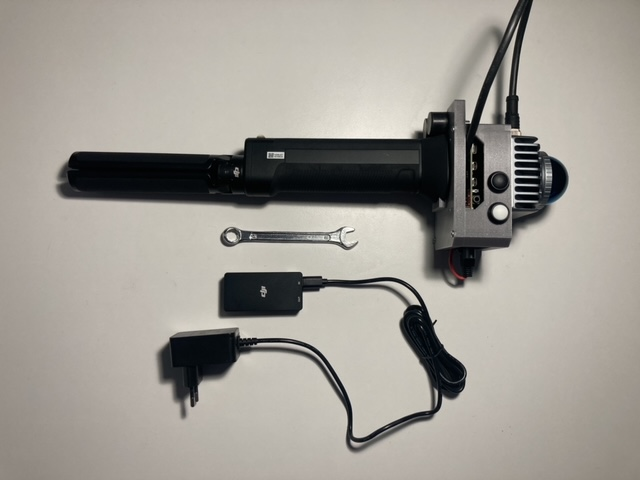
\includegraphics[width=\textwidth, angle = 90]{IMG_9478.jpg}
		\caption{MANDEYE DEV all components - 1: MANDEYE DEV main unit, 2: Handle (attached to main unit), 3:Tripod (attached to handle), 4:Tool for nuts, 5: Charger.}
		\label{fig:m11}
	\end{subfigure}
	\hfill
	\begin{subfigure}[b]{0.7\textwidth}
		\centering
		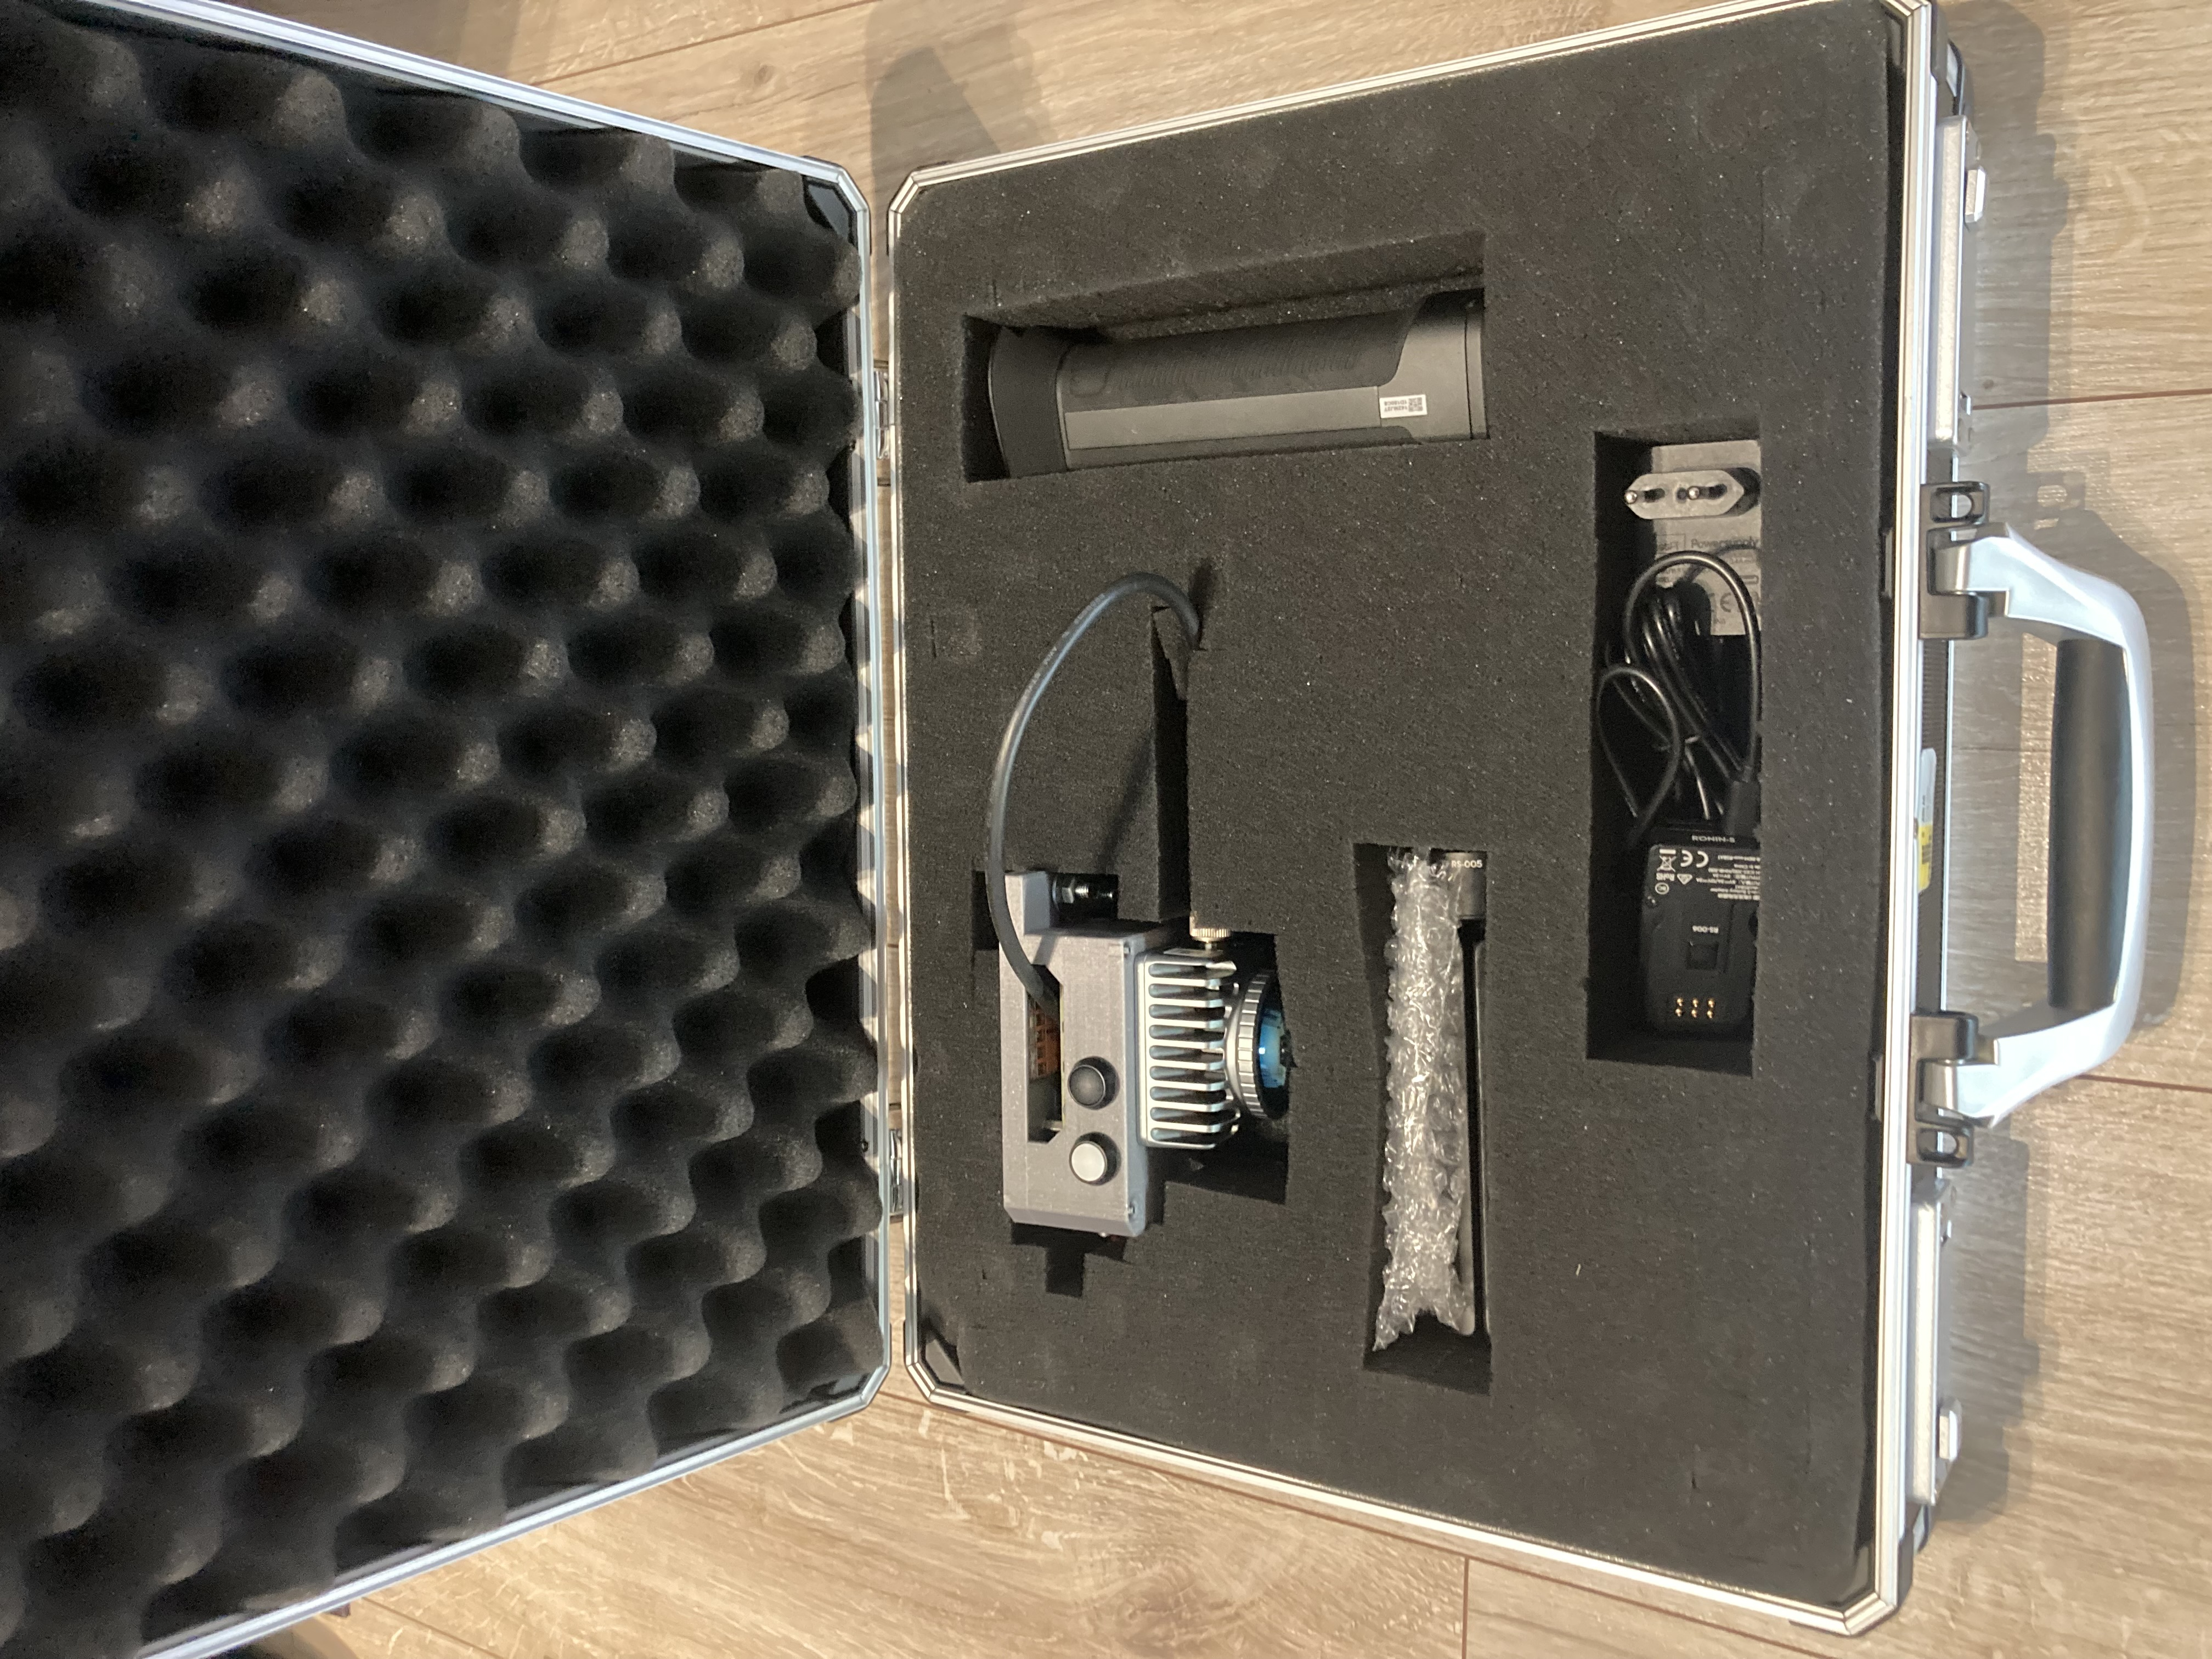
\includegraphics[width=\textwidth, angle = -90]{IMG_9493.jpg}
		\caption{Suitcase with MANDEYE DEV for secure transport.}
		\label{fig:m12}
	\end{subfigure}
	\caption{MANDEYE DEV parts.}
	\label{fig:mandeye_hardware}
\end{figure}

\section{Turn on device}
Please click button on the bottom of the RONIN grip (figure \ref{fig:m21}). 
Green square lights on RONIN grip should be visible. In short time blue light on MANDEYE DEV should be visible indicating that the device is on (figure \ref{fig:m22}). Wait around 30 seconds till all other lights on MANDEYE DEV (green, red and yellow) blink one after another - this indicates that the device is ready for action. Now proceed to Section 2.2 Turn on continuous scanning or to Section 2.4 Turn on stop scan.
Otherwise please check error section \ref{section:errors}.
\begin{figure}[H]
	\centering
	\begin{subfigure}[b]{0.45\textwidth}
		\centering
		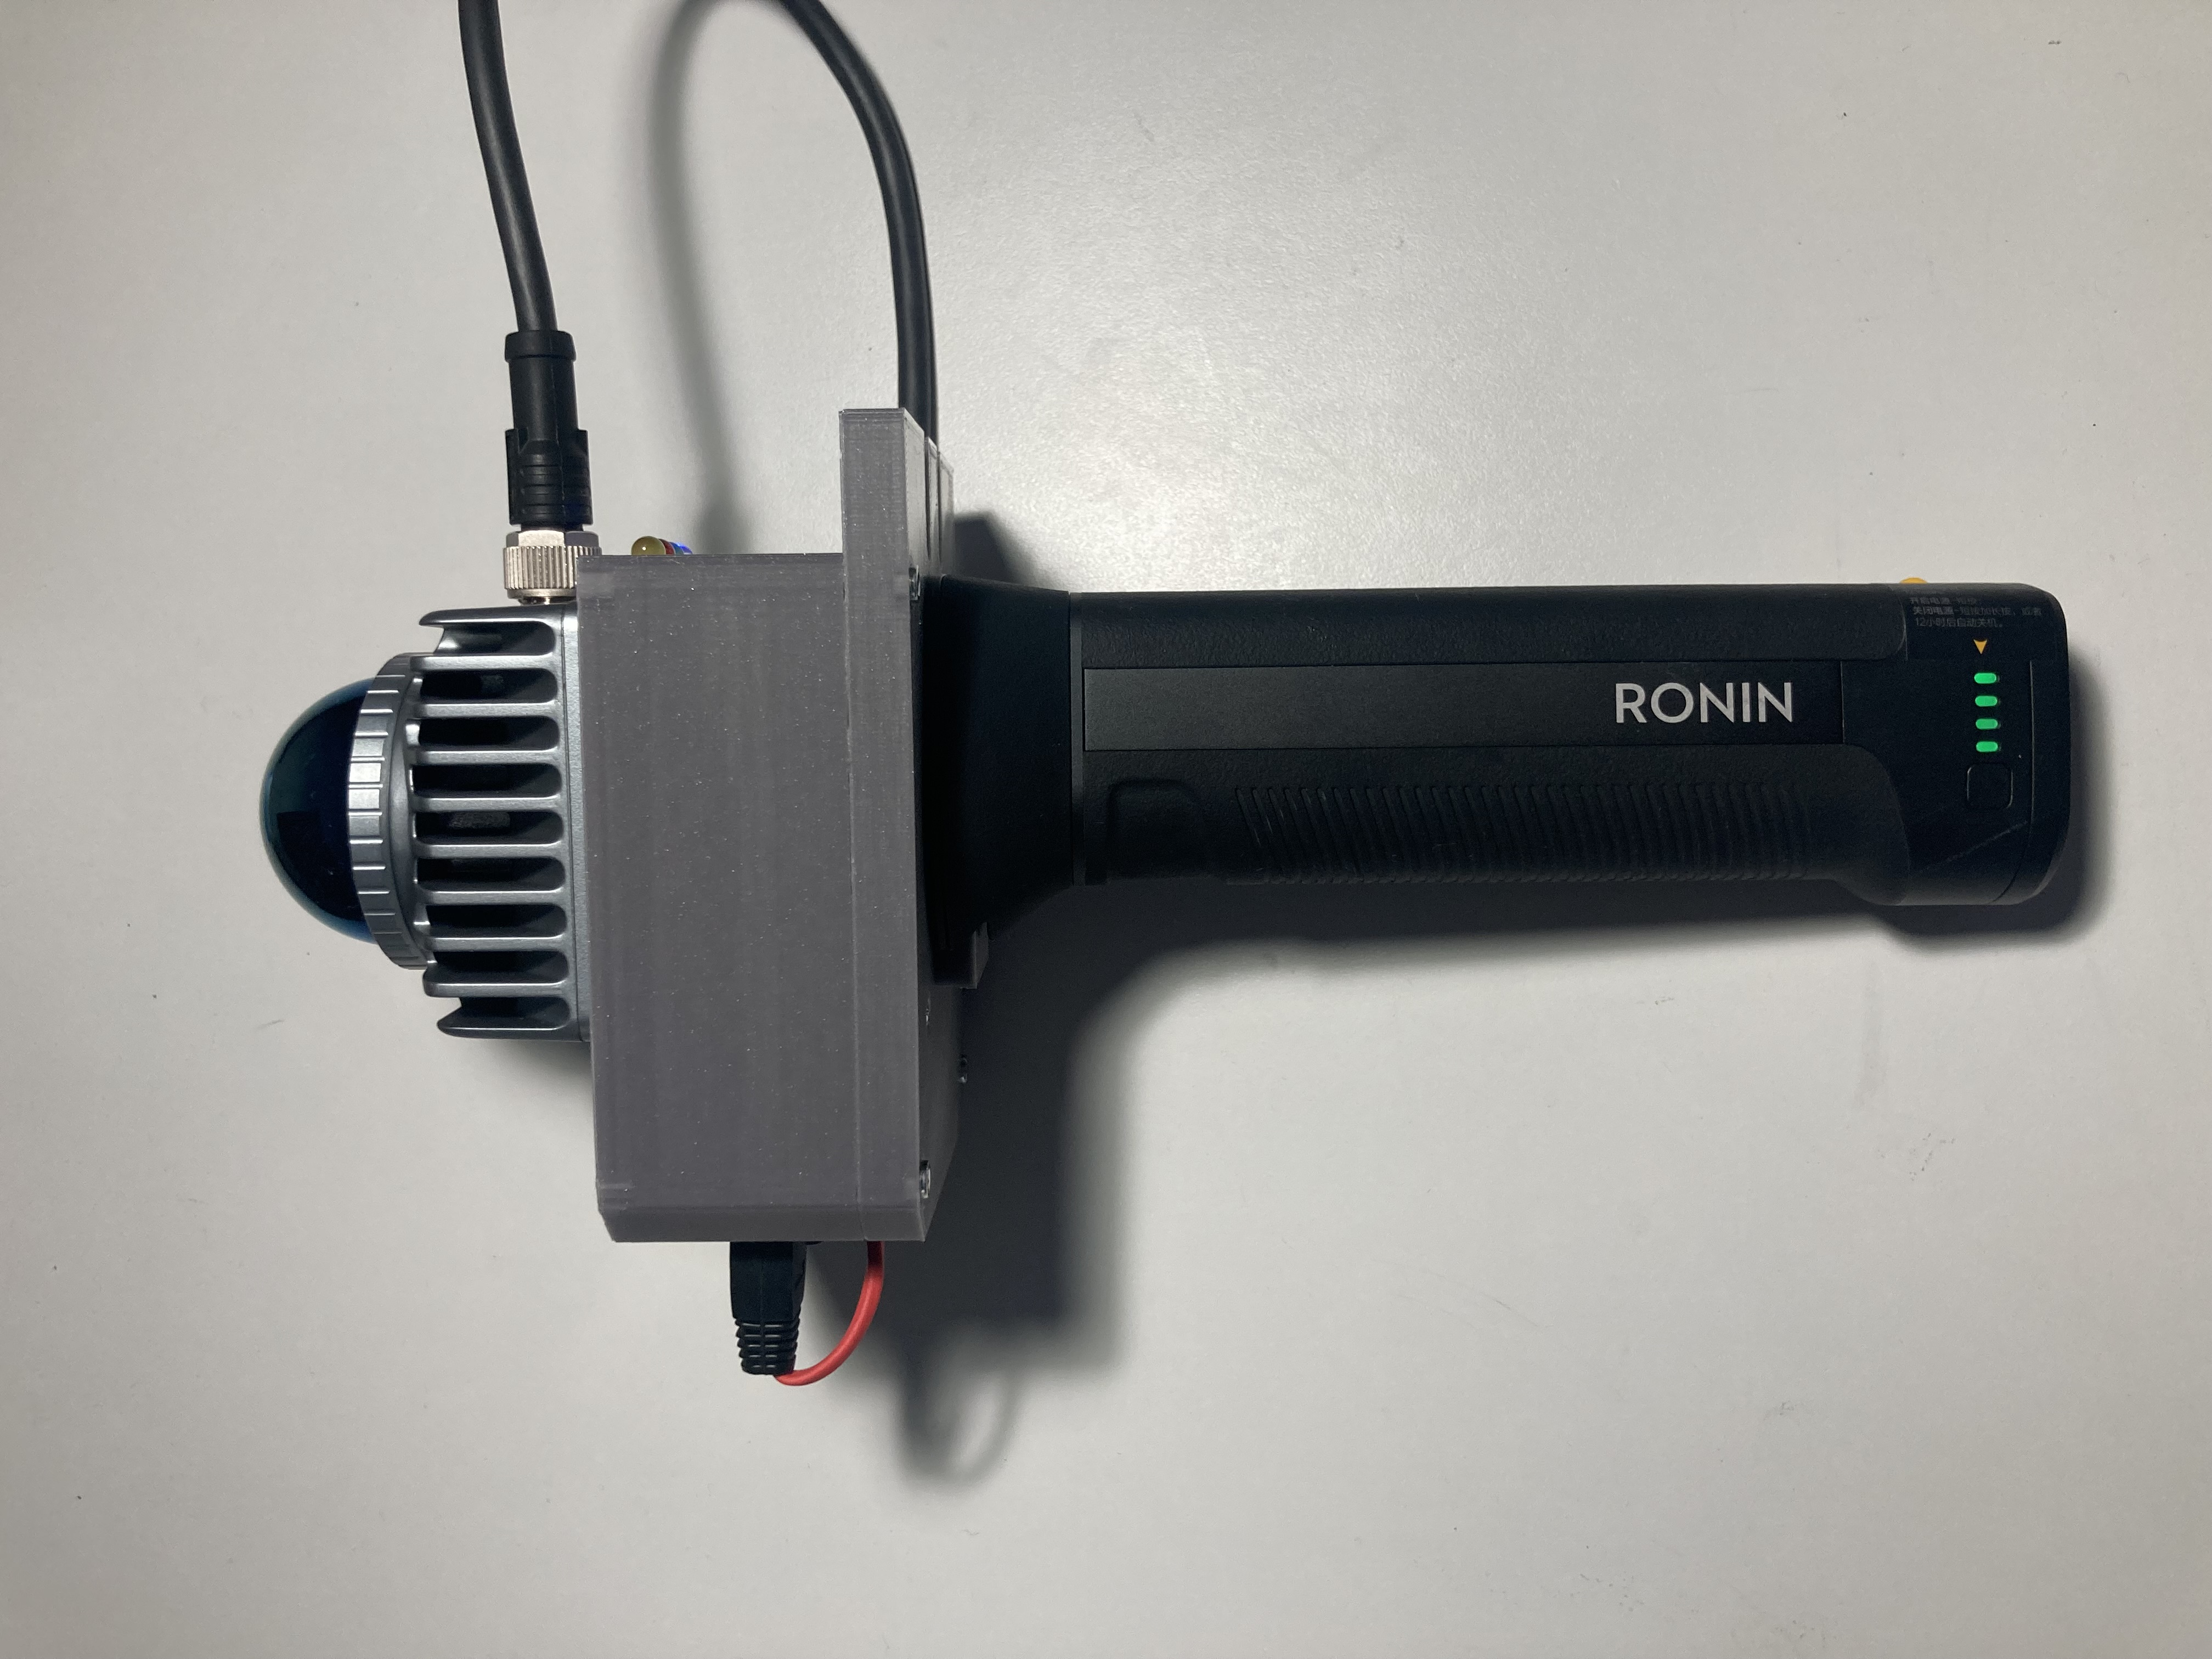
\includegraphics[width=\textwidth, angle = -90]{IMG_9482.jpg}
		\caption{RONIN grip is turned on, green square lights are visible.}
		\label{fig:m21}
	\end{subfigure}
	\hfill
	\begin{subfigure}[b]{0.45\textwidth}
		\centering
		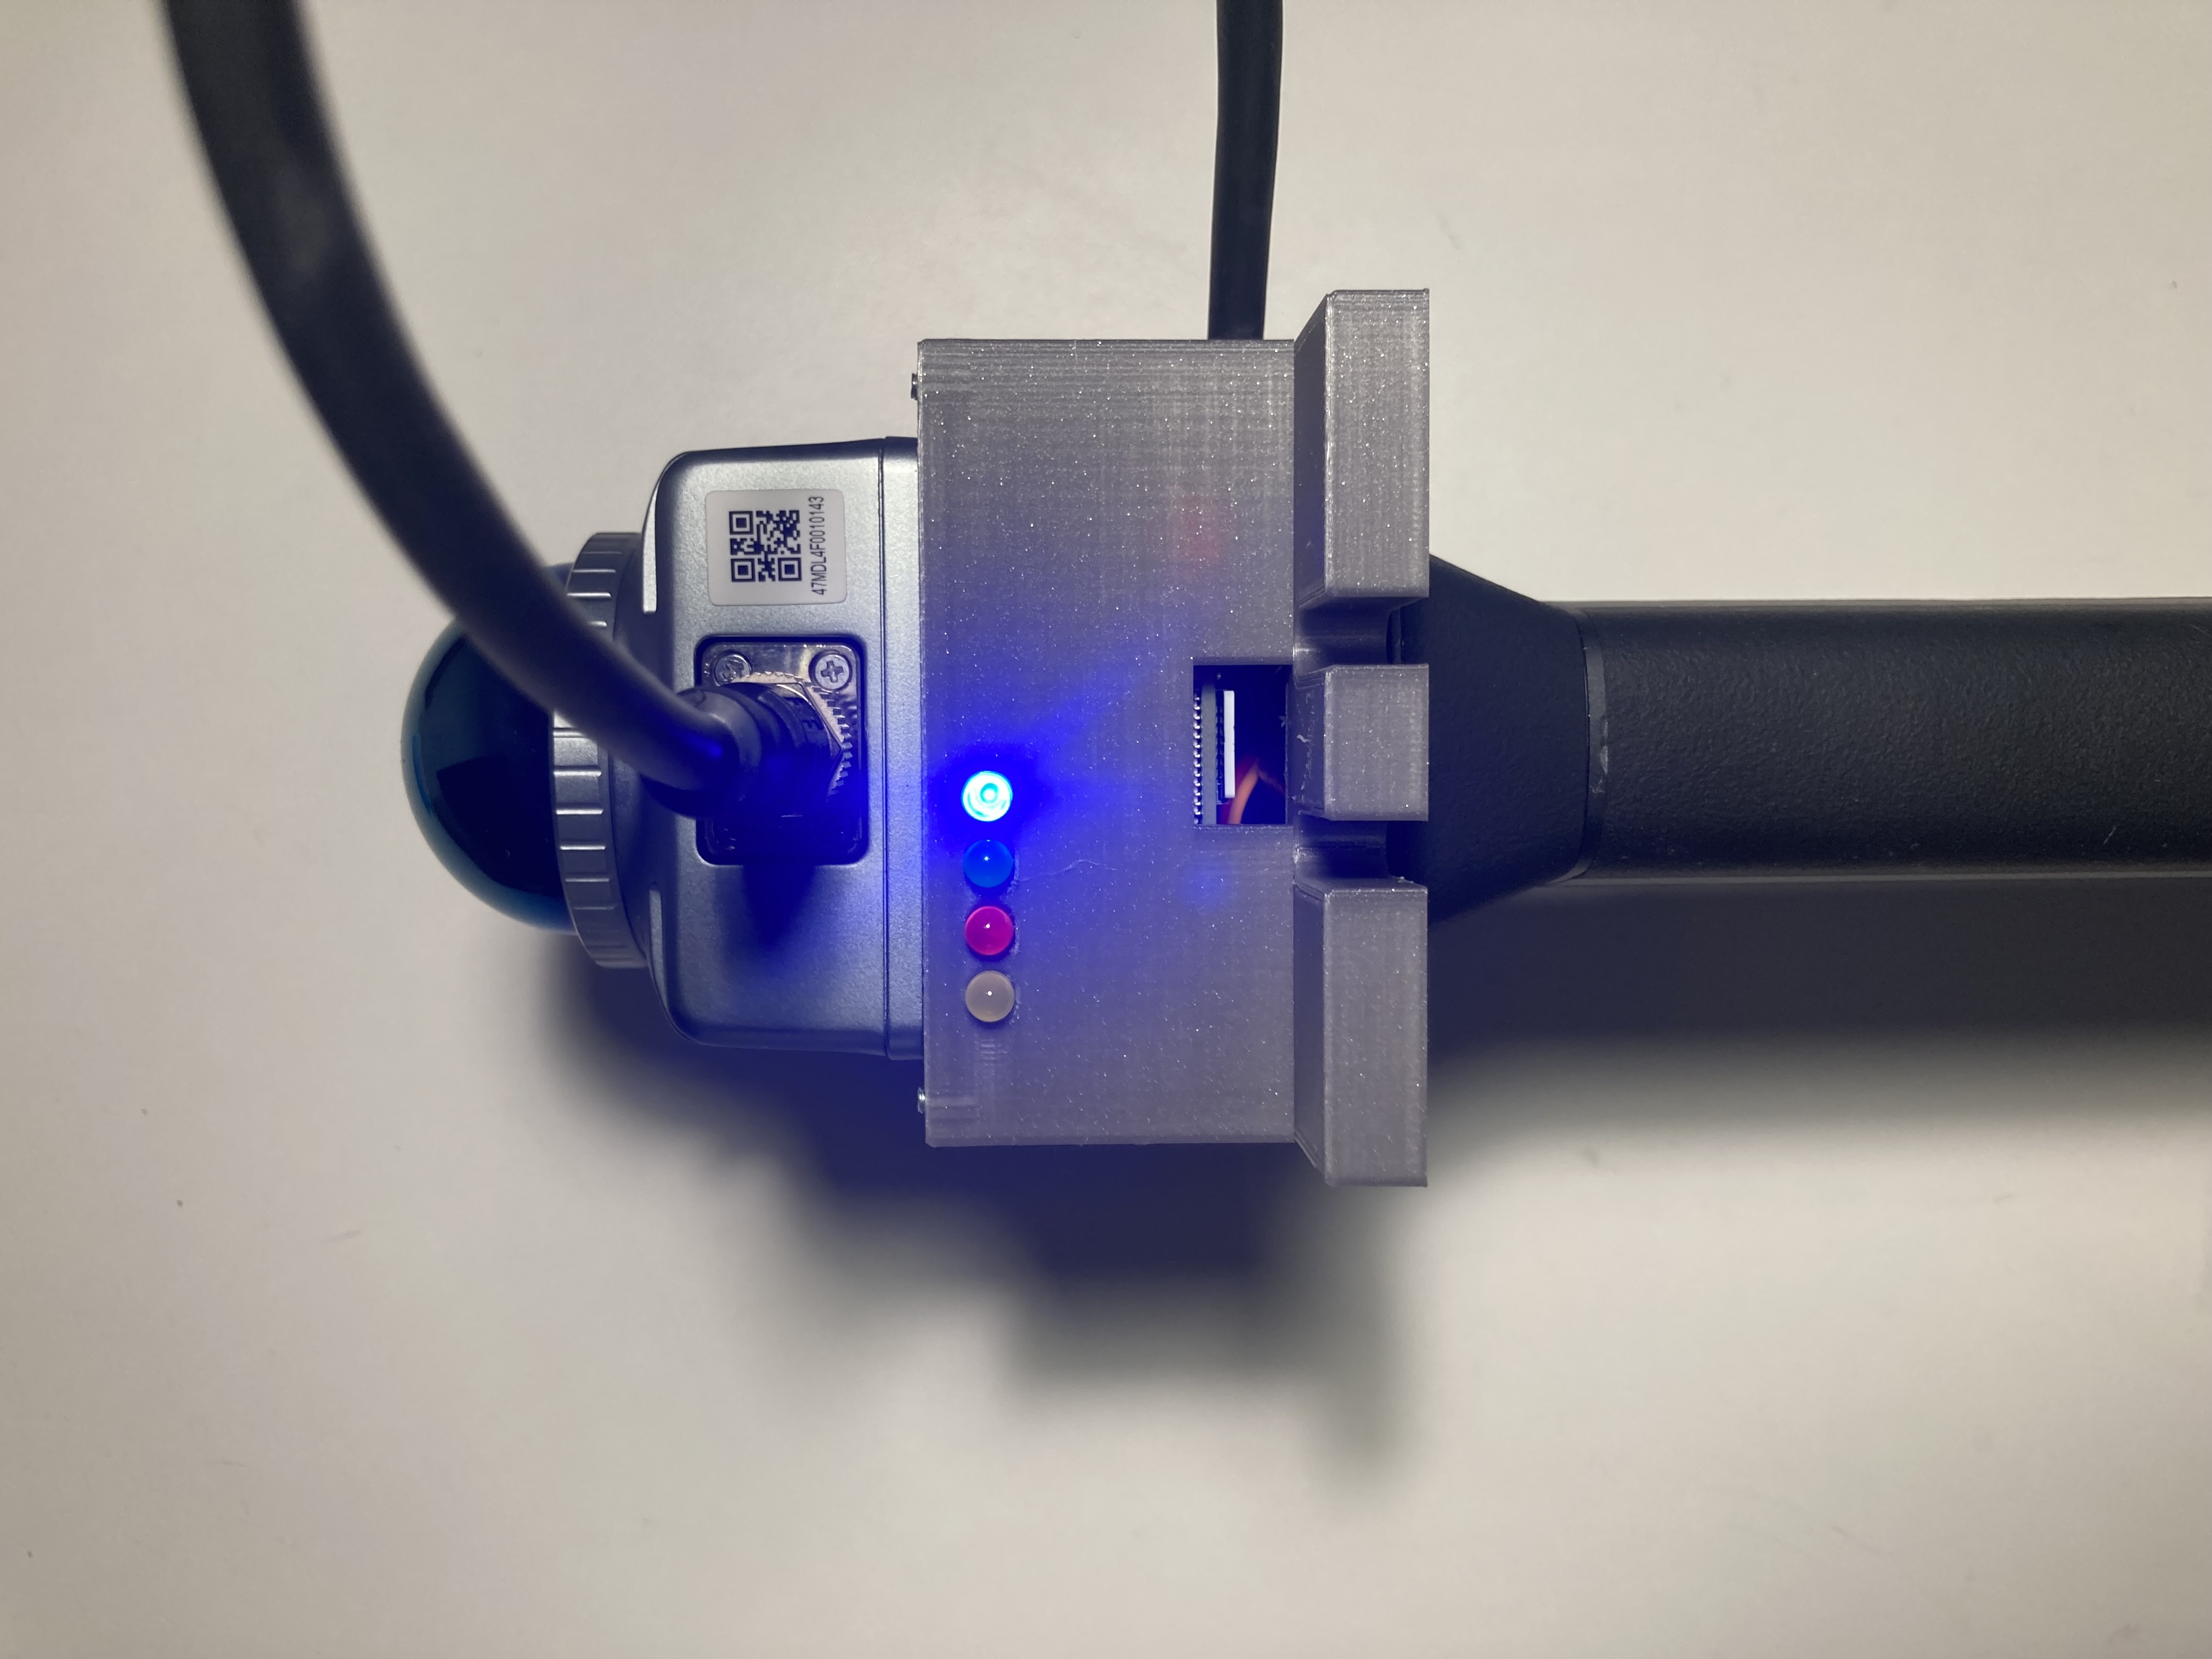
\includegraphics[width=\textwidth, angle = -90]{IMG_9484.jpg}
		\caption{MANDEYE DEV is turned on, blue light can be seen.}
		\label{fig:m22}
	\end{subfigure}
	\caption{MANDEYE DEV turned on.}
	\label{fig:mandeye_hardware2}
\end{figure}
\section{Turn on continuous scanning}
If everything from section 2.1 is done and no errors where indicated (otherwise check error section \ref{section:errors}) the procedure for running continuous data collection is as follows:
\begin{itemize}
	\item 1: Place MANDEYE DEV steady on the ground using attached tripod.
	\item 2: \begin{minipage}[t]{\linewidth}
		\raggedright
		\adjustbox{valign=t}{%
		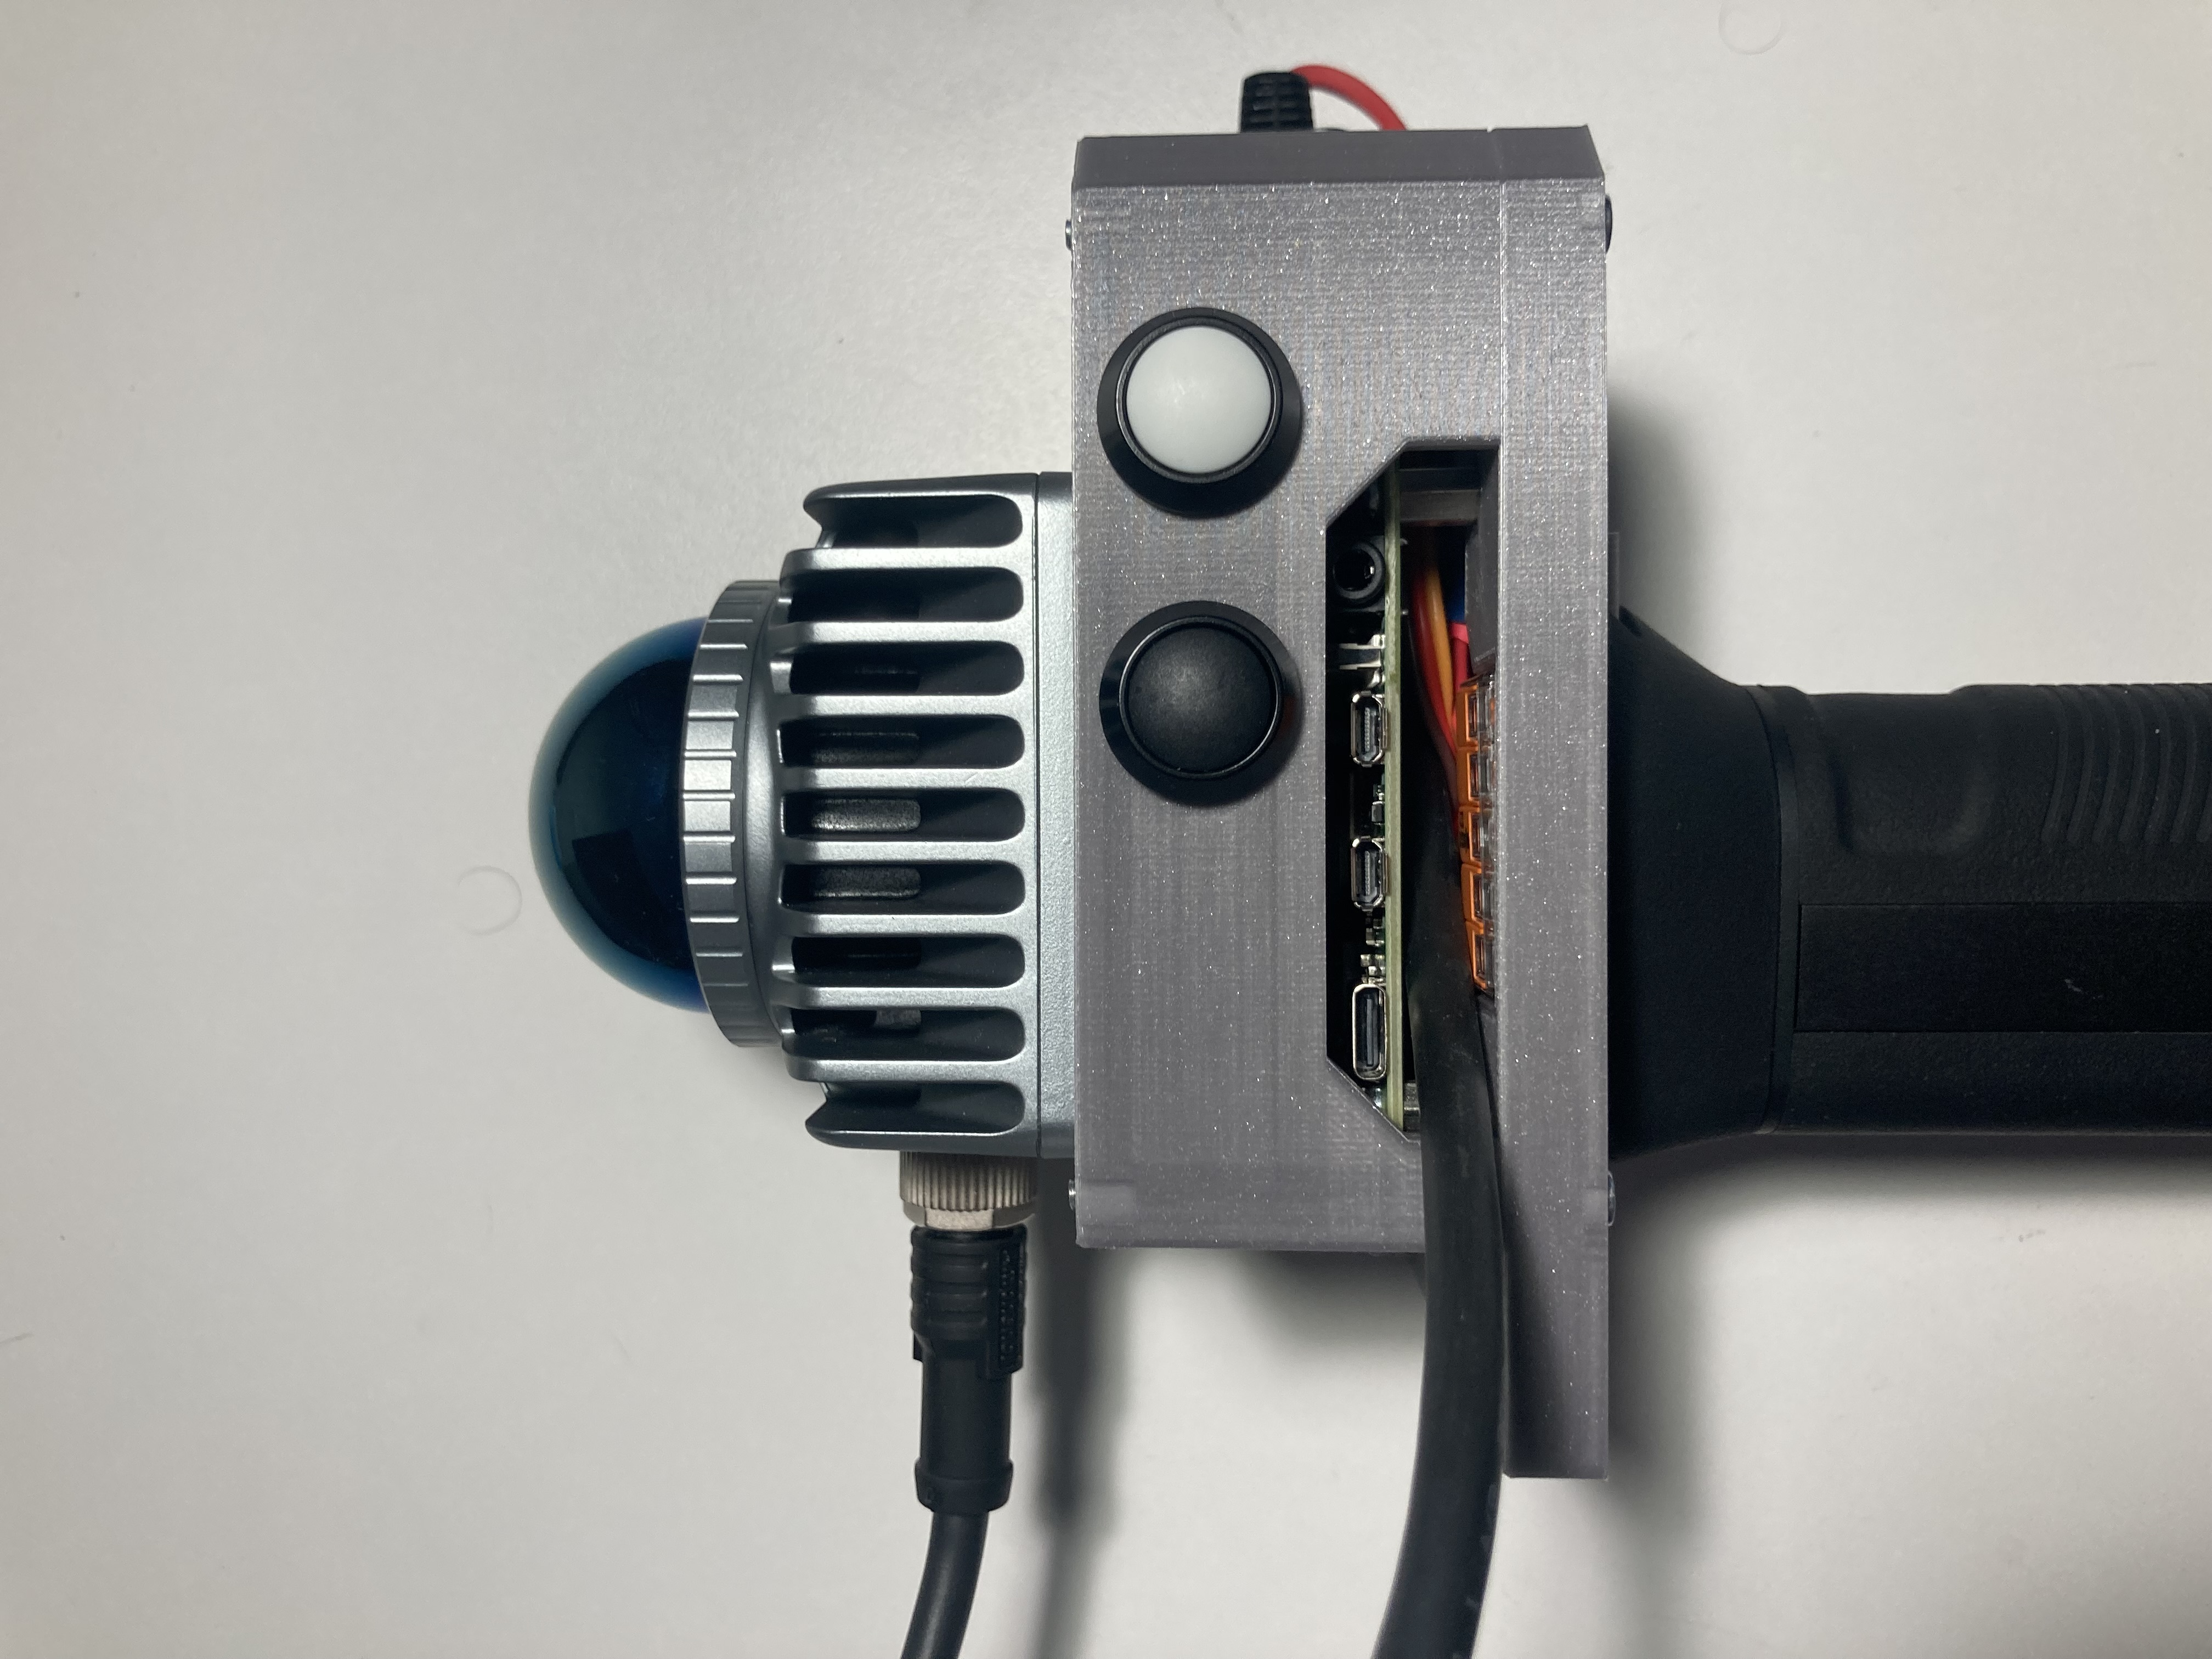
\includegraphics[width=\textwidth, angle = -90]{IMG_9481.jpg}%
		}		
		\medskip	
	\end{minipage}
	Push white button, after doing so green light should turn on (figure \ref{fig:m31}). 
	\item 3: Gently take MANDEYE DEV to hand and go around your scanning area.
	\item 4: Go back to starting point (if possible) and gently place MANDEYE DEV on the ground.
	\item 5: To turn off continuous scanning push white button while red light (figure \ref{fig:m32}) is not indicating the fact that device is copying data from local memory to USB drive. After that green light should turn off leaving only the blue light on. MANDEYE DEV is again in the ready for action state (blue light is on and scanning can be started).
\end{itemize}
\begin{figure}[H]
	\centering
	\begin{subfigure}[b]{0.45\textwidth}
		\centering
		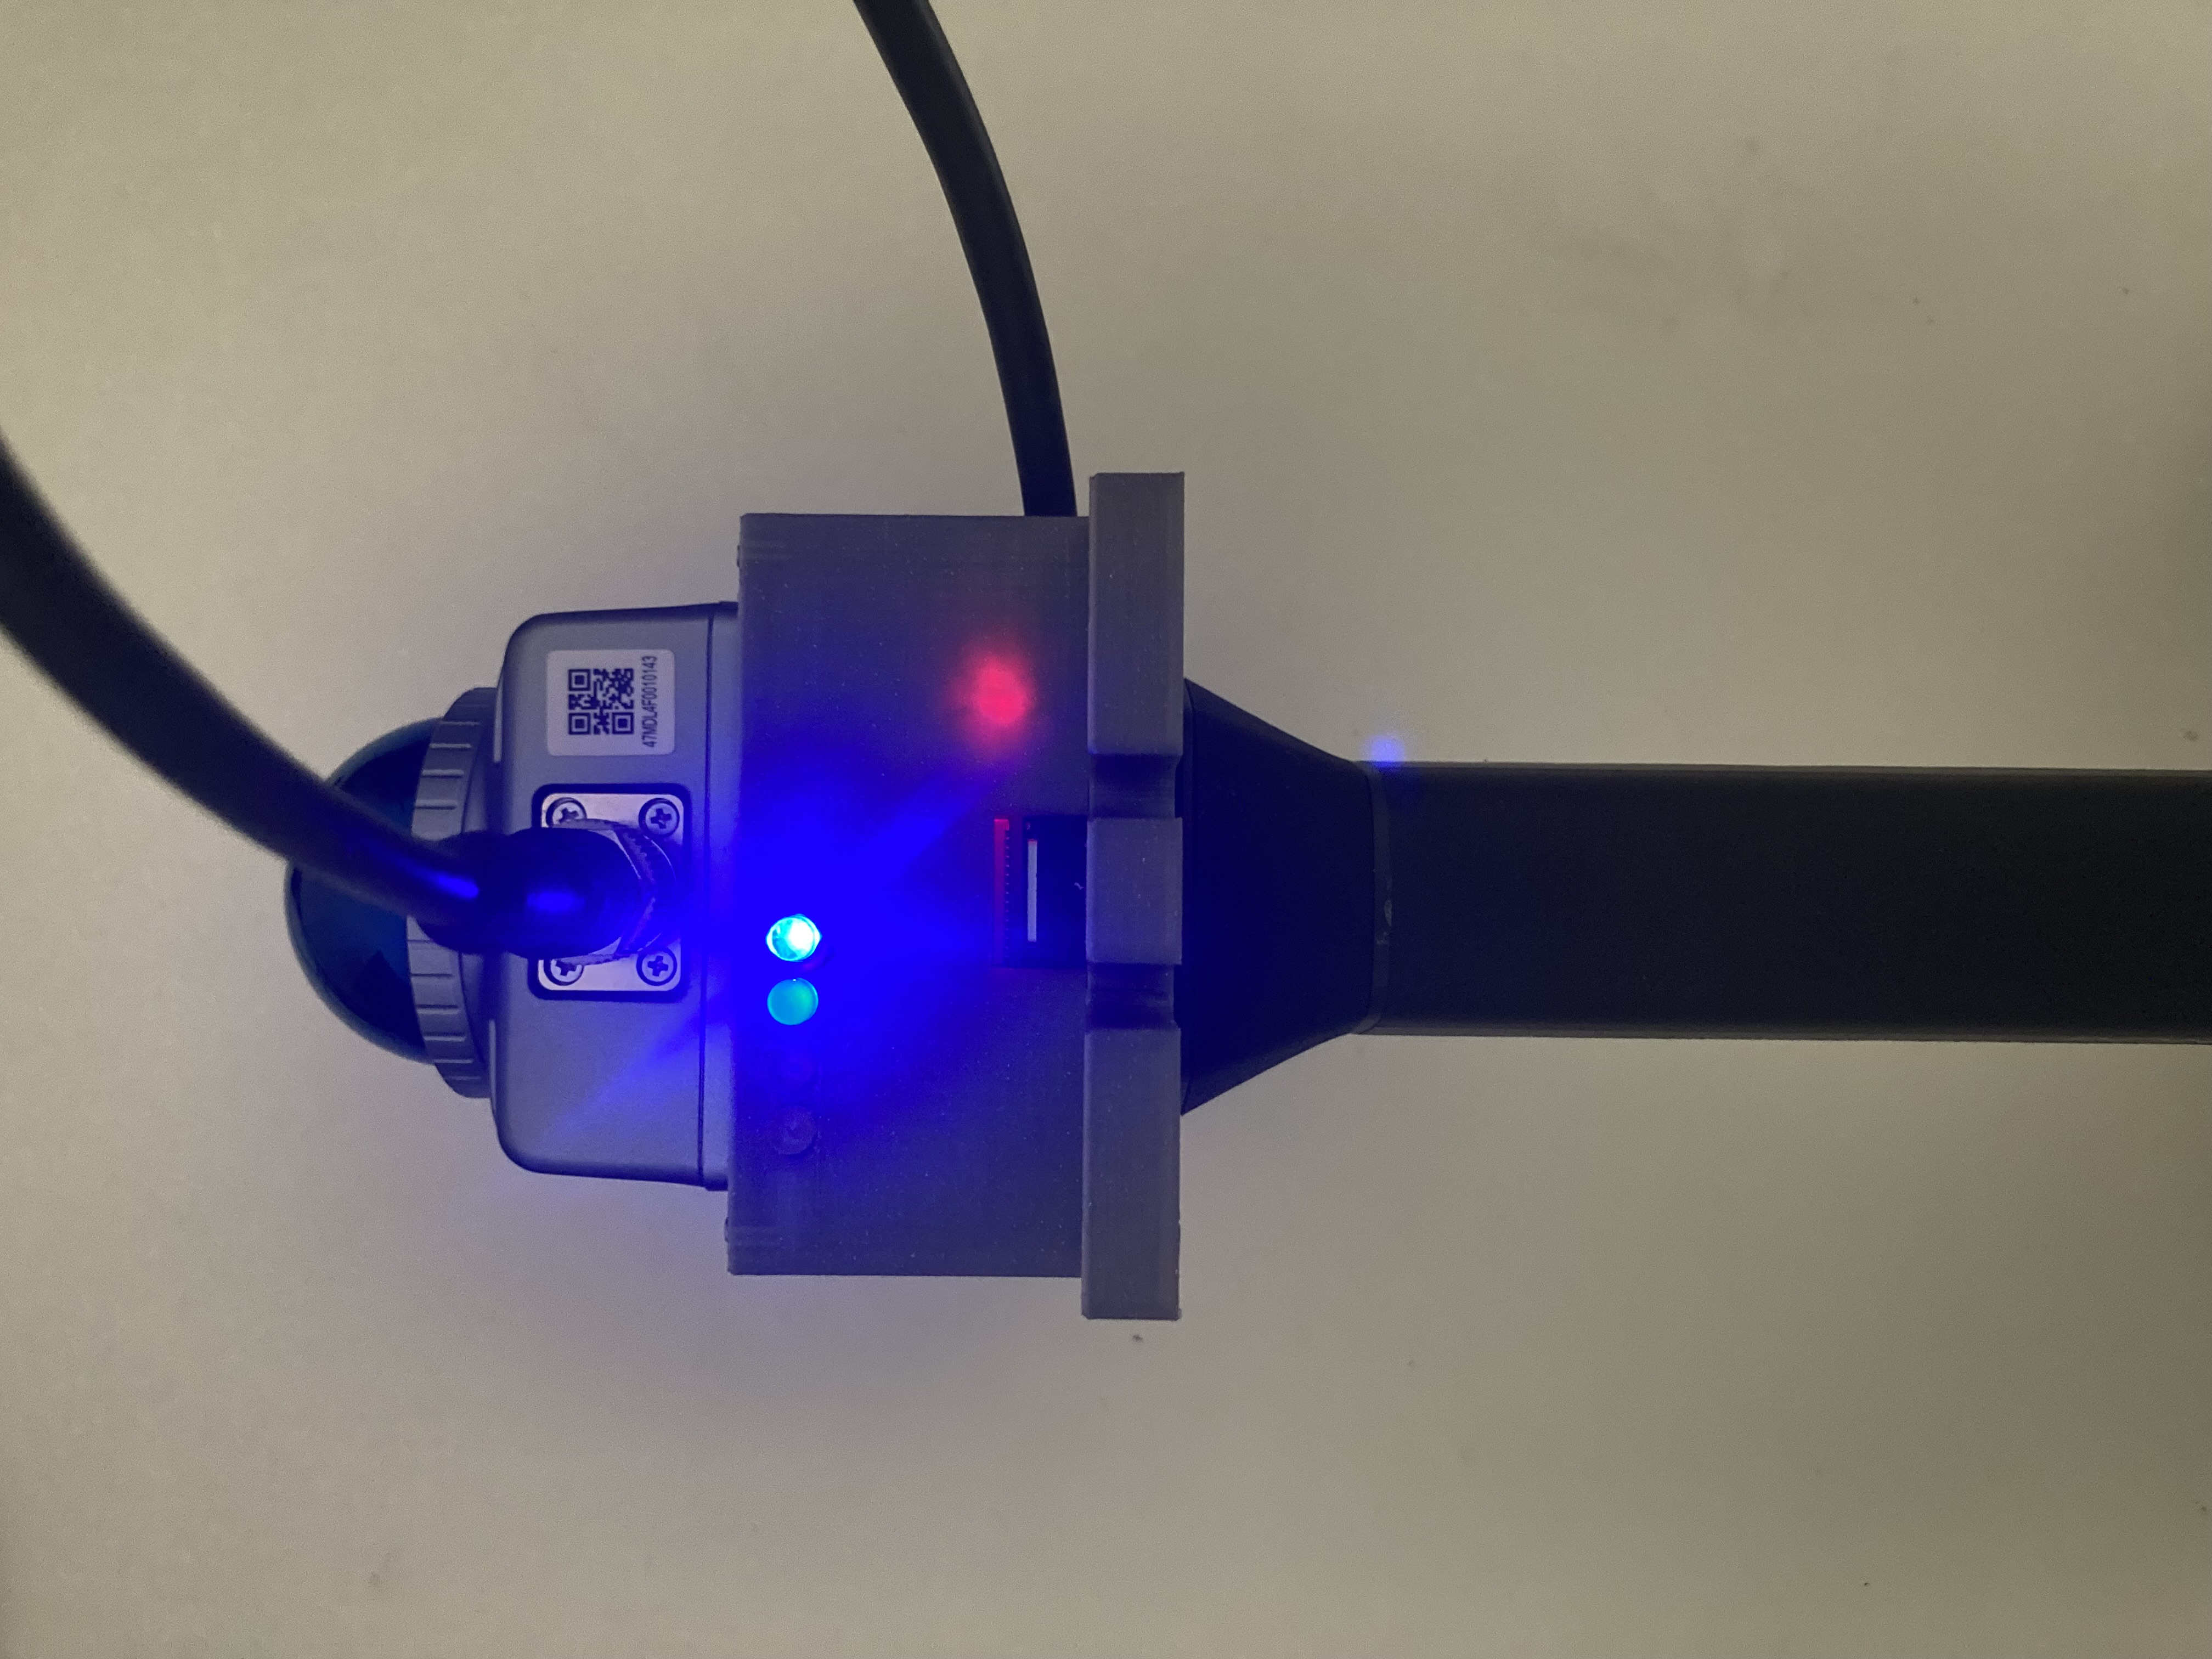
\includegraphics[width=\textwidth, angle = -90]{IMG_9494.jpg}
		\caption{MANDEYE DEV is showing by green light that 3D continuous scanning data are recorded in local memory.}
		\label{fig:m31}
	\end{subfigure}
	\hfill
	\begin{subfigure}[b]{0.45\textwidth}
		\centering
		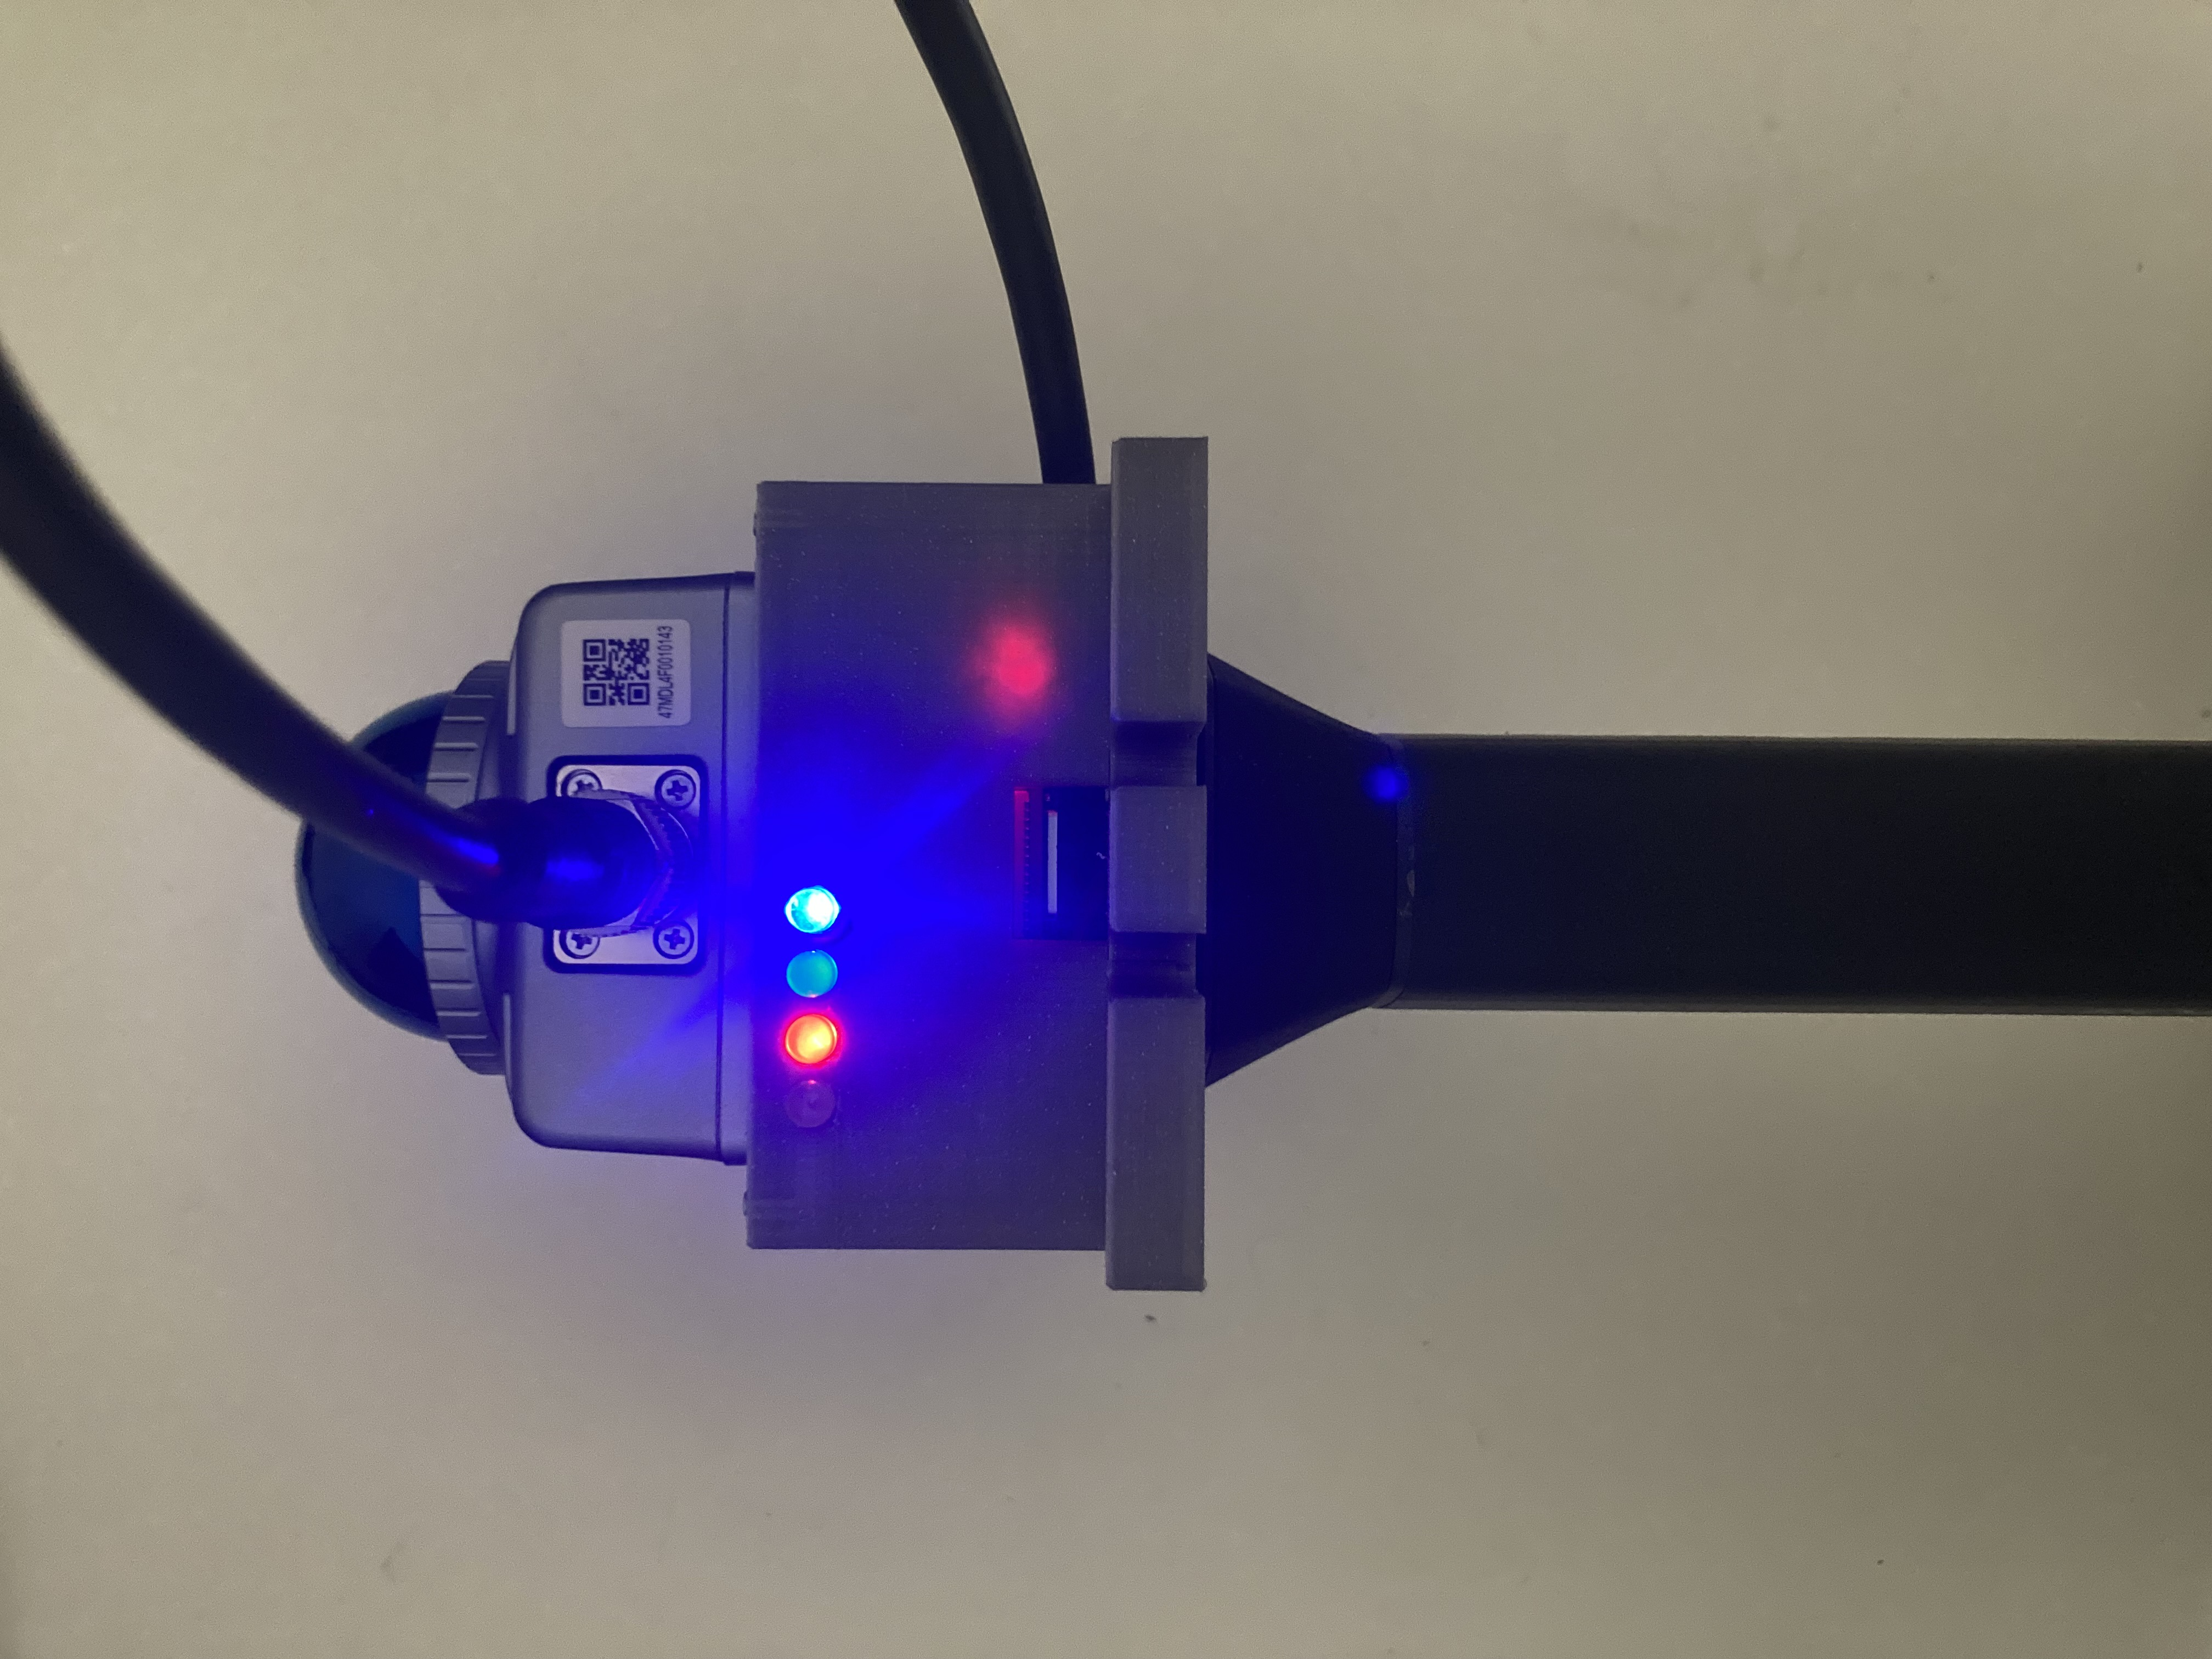
\includegraphics[width=\textwidth, angle = -90]{IMG_9495.jpg}
		\caption{MANDEYE DEV is showing by green and red light that it copies continuous scanning data from local memory to USB stick.}
		\label{fig:m32}
	\end{subfigure}
	\caption{MANDEYE DEV during continuous scanning.}
	\label{fig:mandeye_hardware3}
\end{figure}

\pagebreak
\section{Turn on stop scan}
If everything from section 2.1 is done and no errors where indicated (otherwise check error section \ref{section:errors}) the procedure for using stop scan is as follows:
\begin{itemize}
	\item 1a: Place MANDEYE DEV steady on the ground.
	\item 2a: \begin{minipage}[t]{0.75\linewidth}
		\raggedright
		\adjustbox{valign=t}{%
			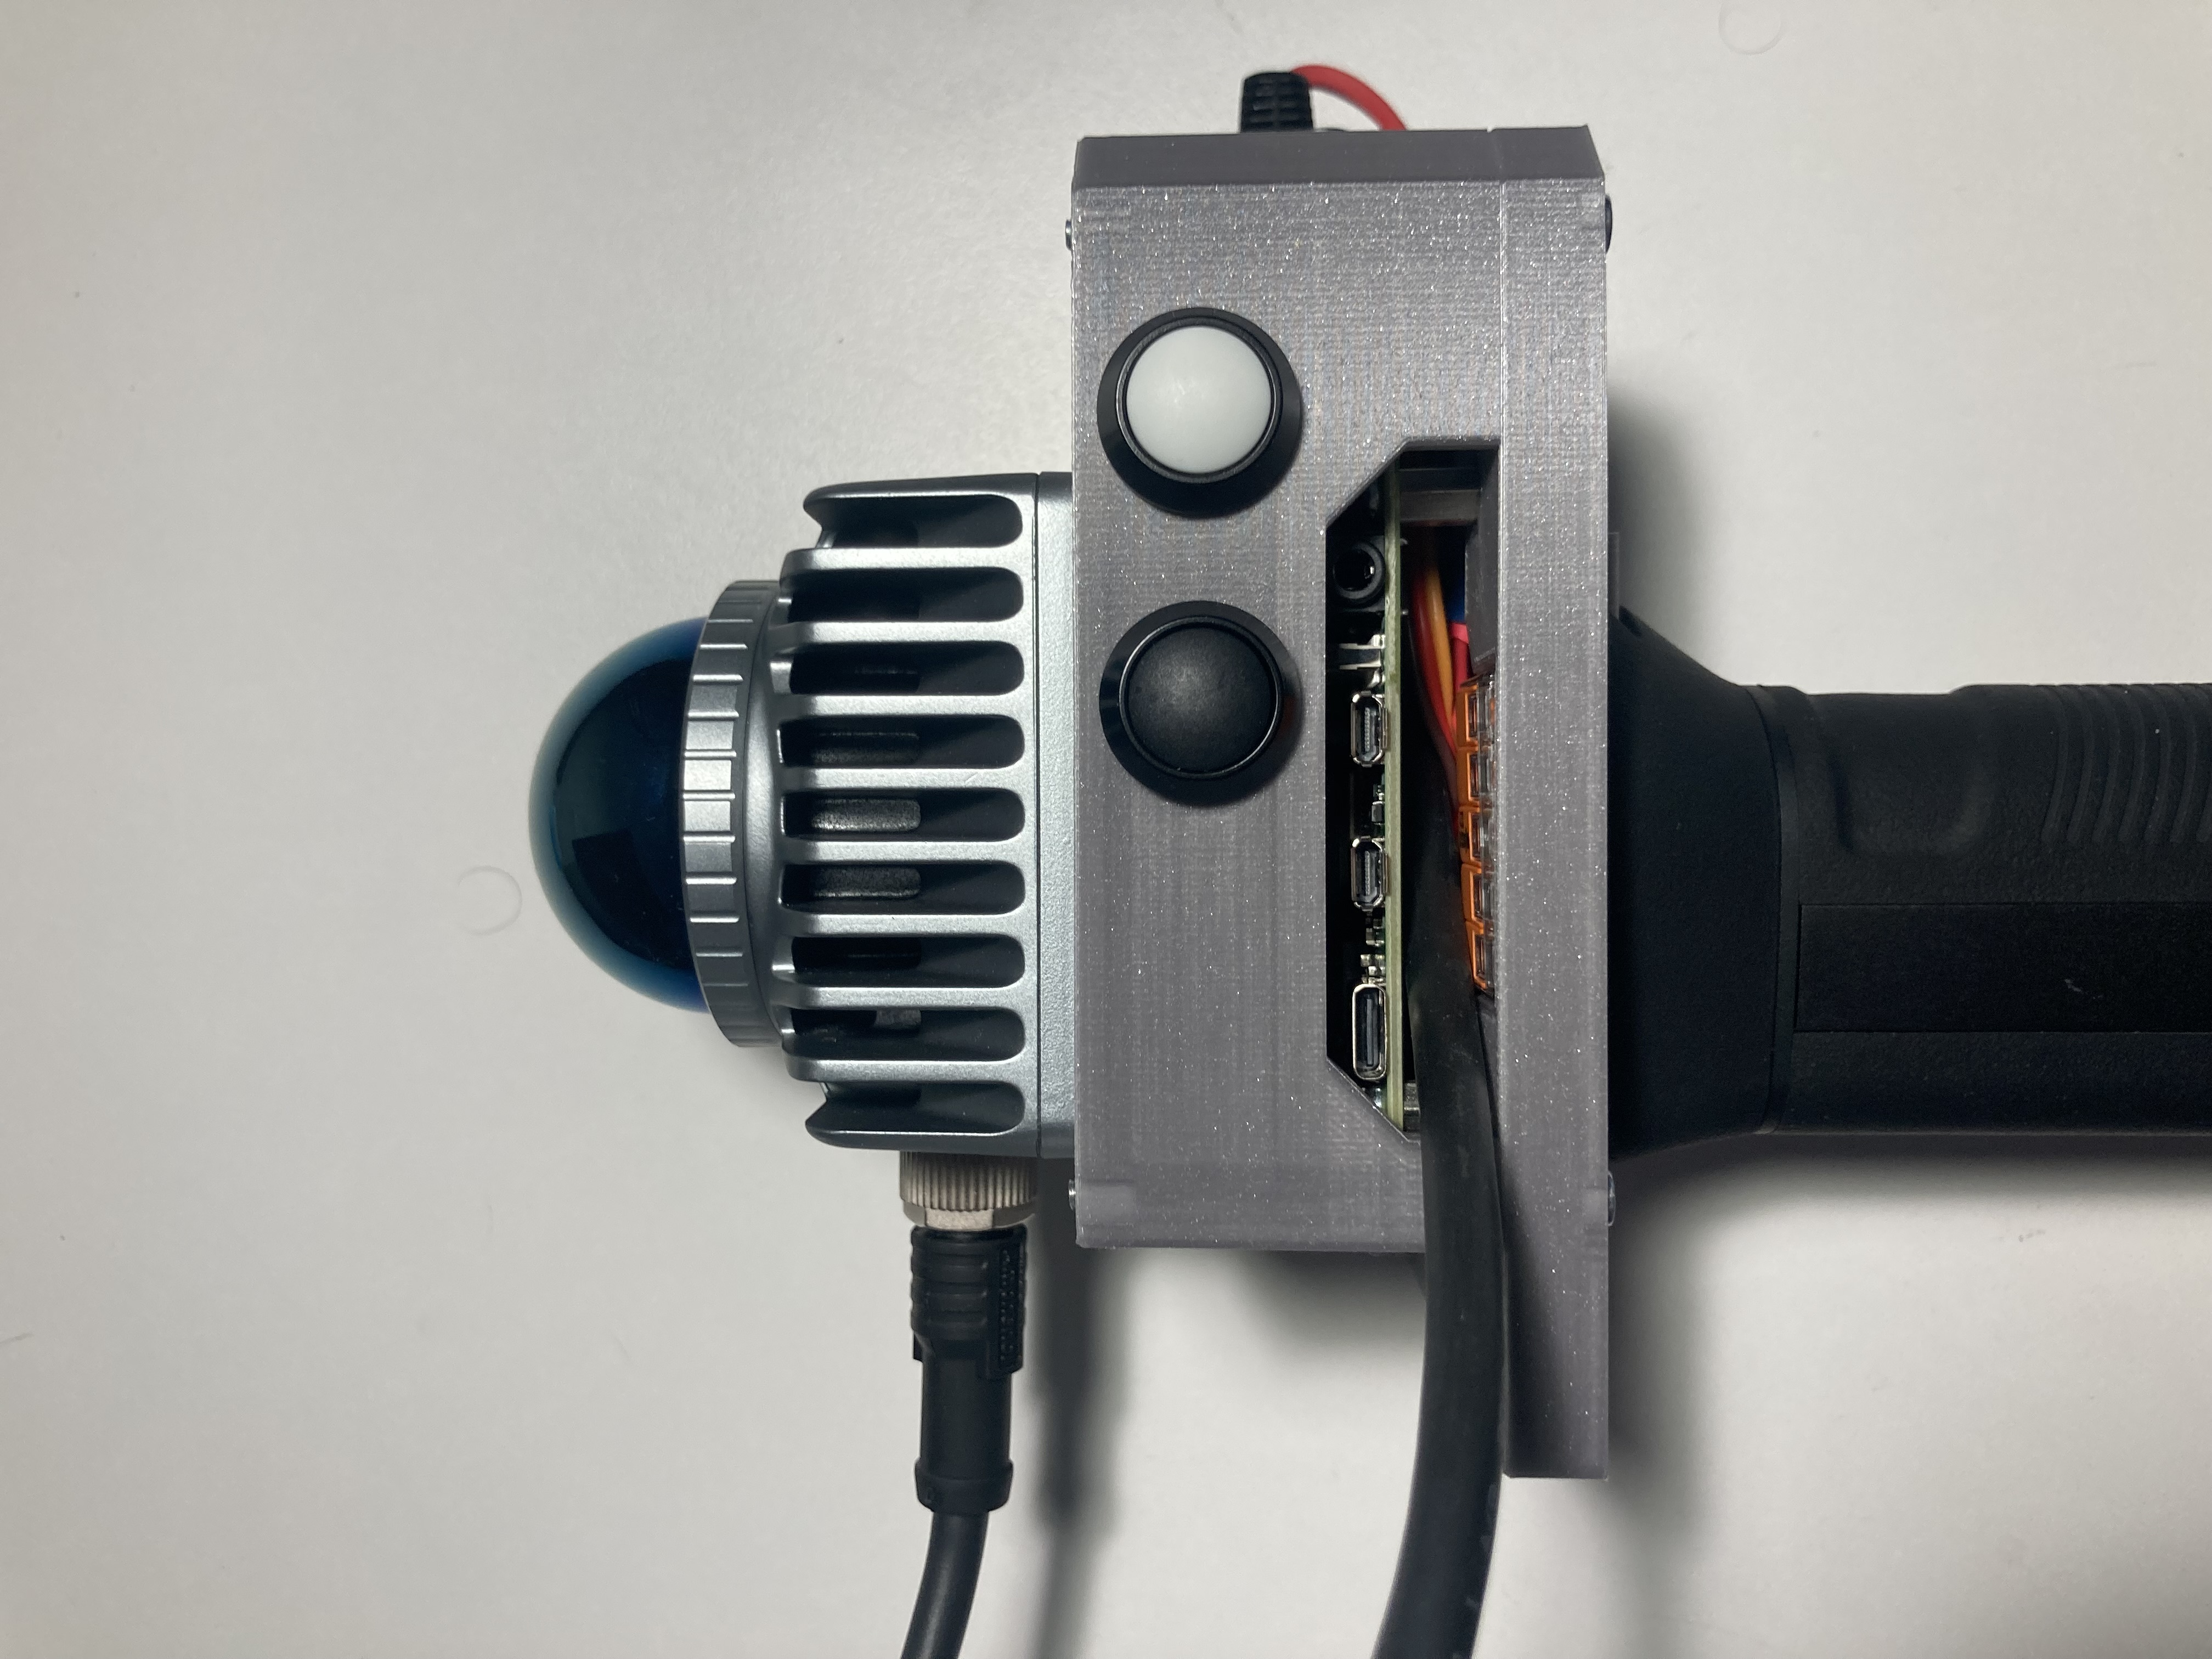
\includegraphics[width=\textwidth, angle = -90]{IMG_9481.jpg}%
		}		
		\medskip	
	\end{minipage}
	\linebreak
	Push black button and wait till yellow and red lights (figure \ref{fig:m42}) will turn off.
	\item 1b: Place MANDEYE DEV steady on the ground in second location.
	\item 2b: Push black button and wait till yellow and red lights will turn off.
	\item 1c: Place MANDEYE DEV steady on the ground in third location.
	\item 2c: Push black button and wait till yellow and red lights will turn off.
	\item 1d: ...
	\item 2d: ...
	\item 1N: Place MANDEYE DEV steady on the ground in N-th location.
	\item 2N: Push black button and wait till yellow and red lights will turn off.
\end{itemize}
\begin{figure}[H]
	\centering
	\begin{subfigure}[b]{0.45\textwidth}
		\centering
		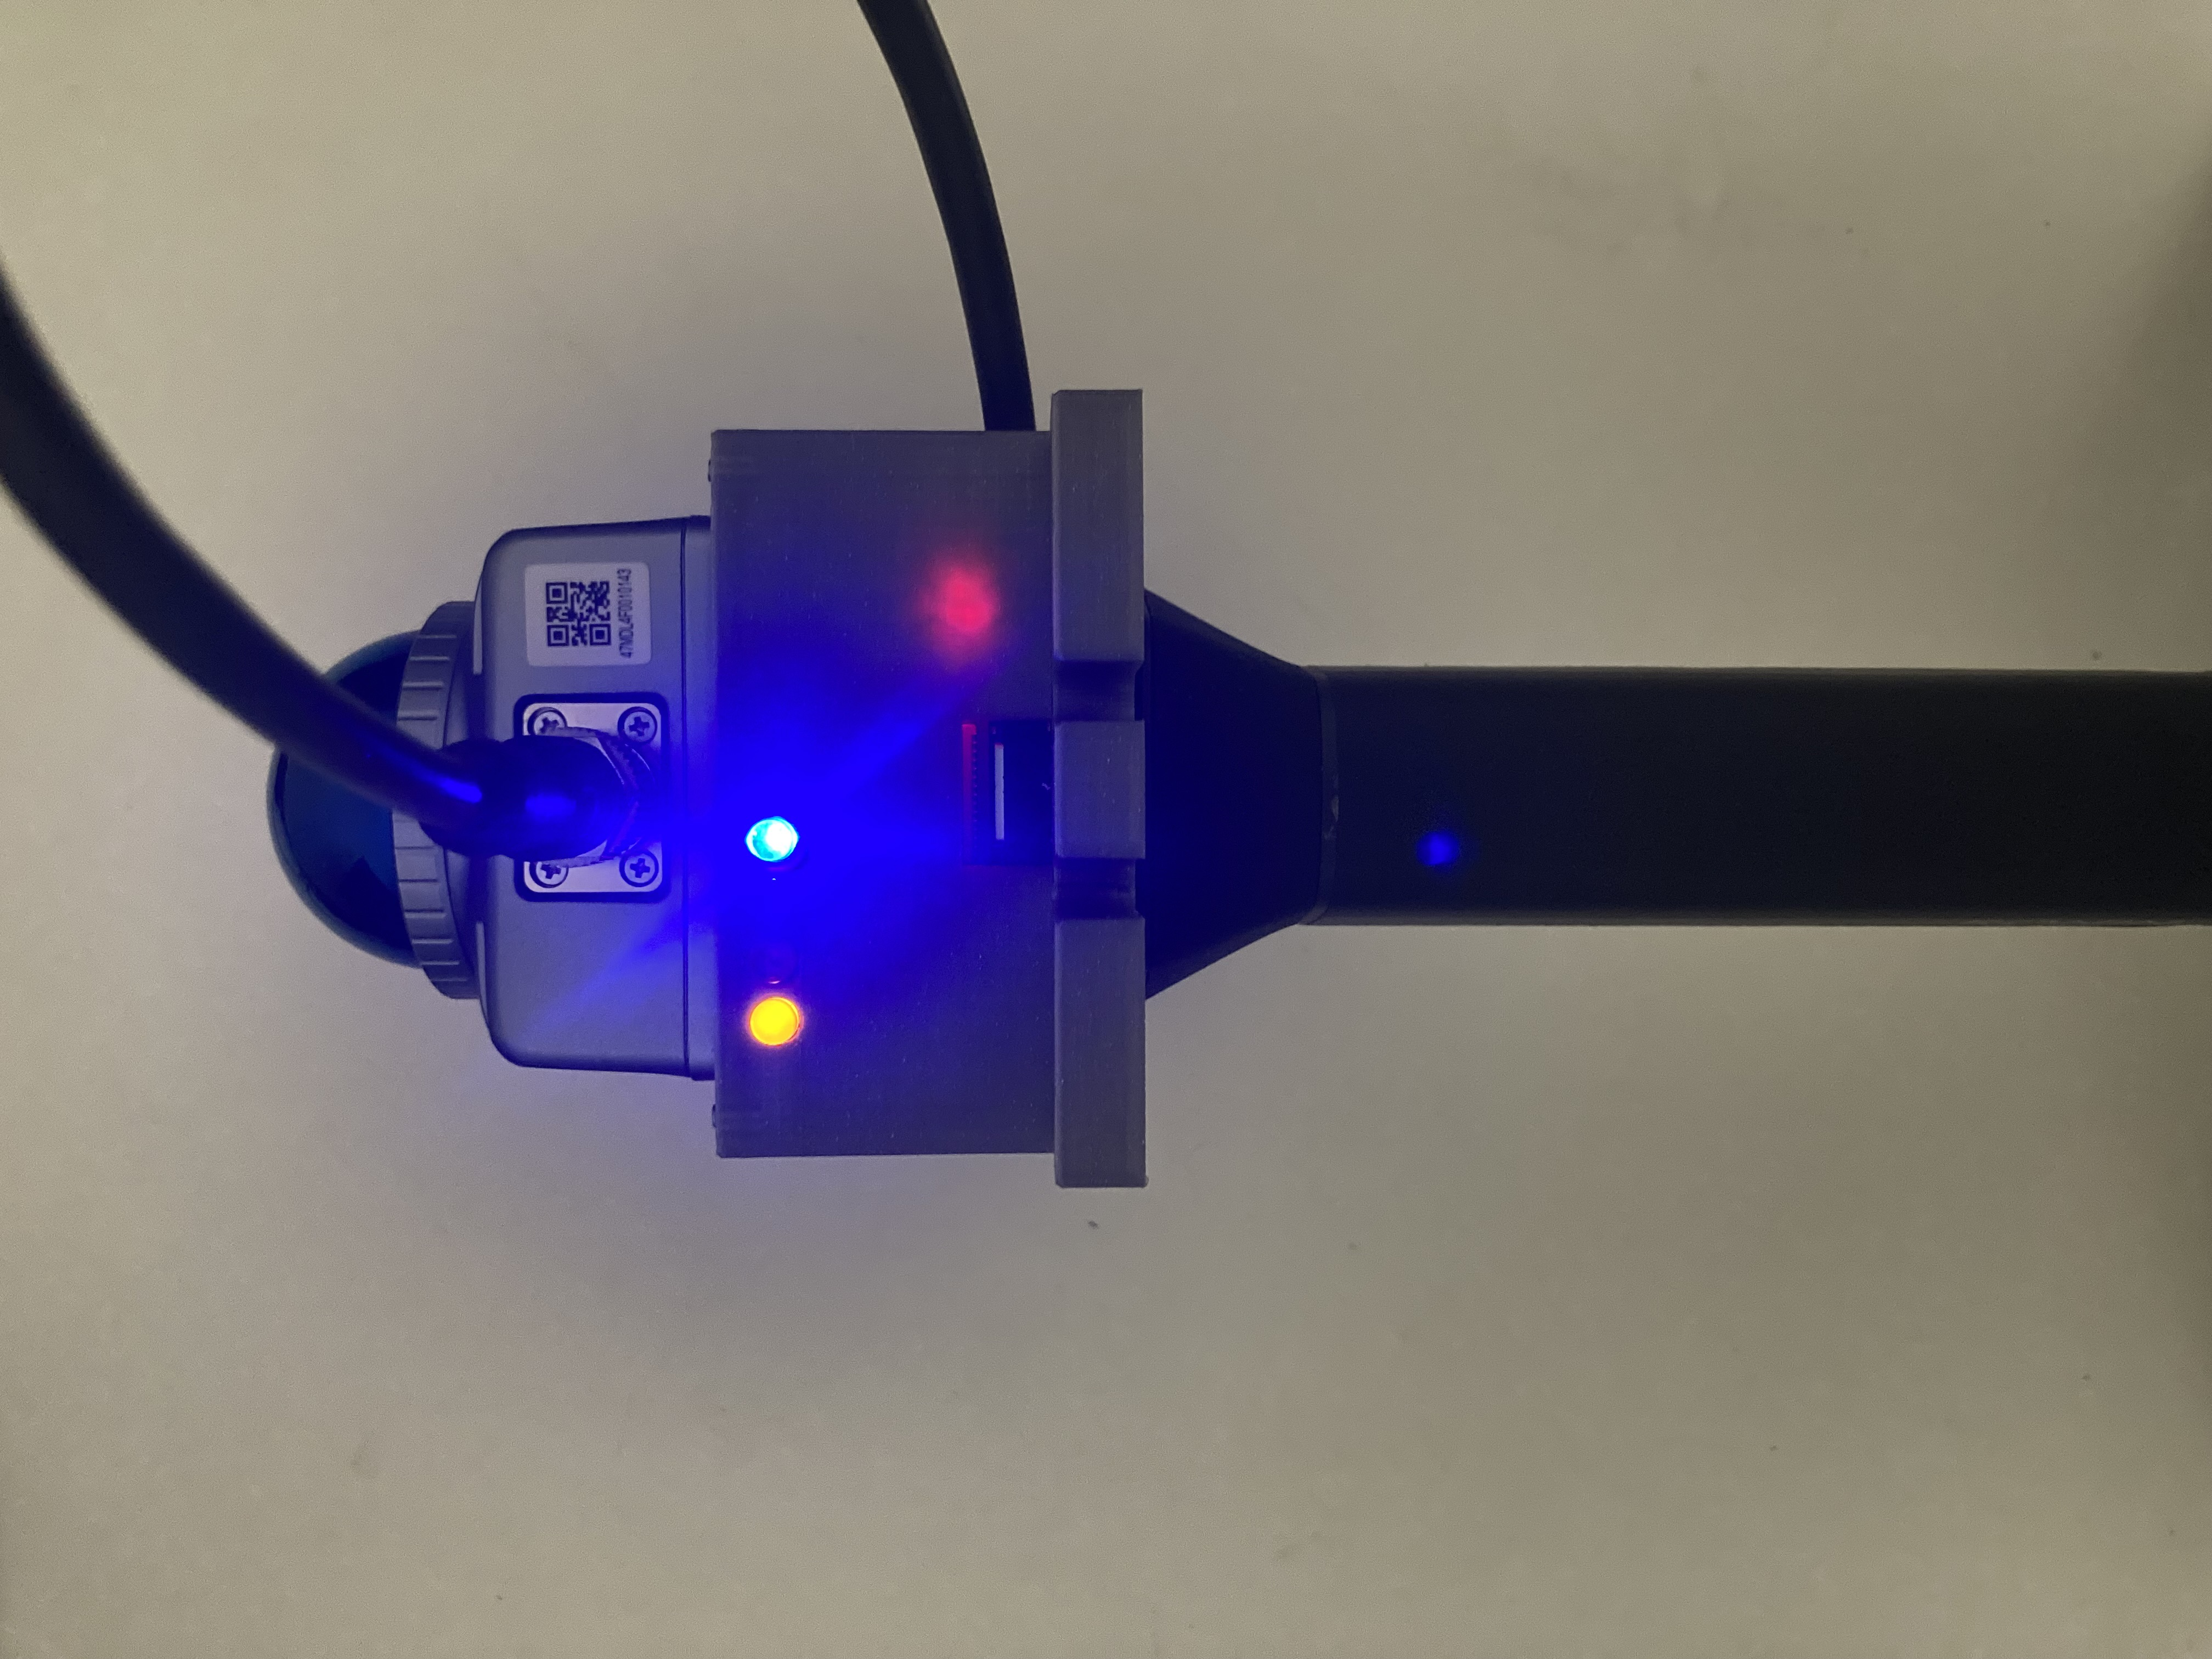
\includegraphics[width=\textwidth, angle = -90]{IMG_9498.jpg}
		\caption{MANDEYE DEV is showing by yellow light that 3D data are recorded in local memory.}
		\label{fig:m41}
	\end{subfigure}
	\hfill
	\begin{subfigure}[b]{0.45\textwidth}
		\centering
		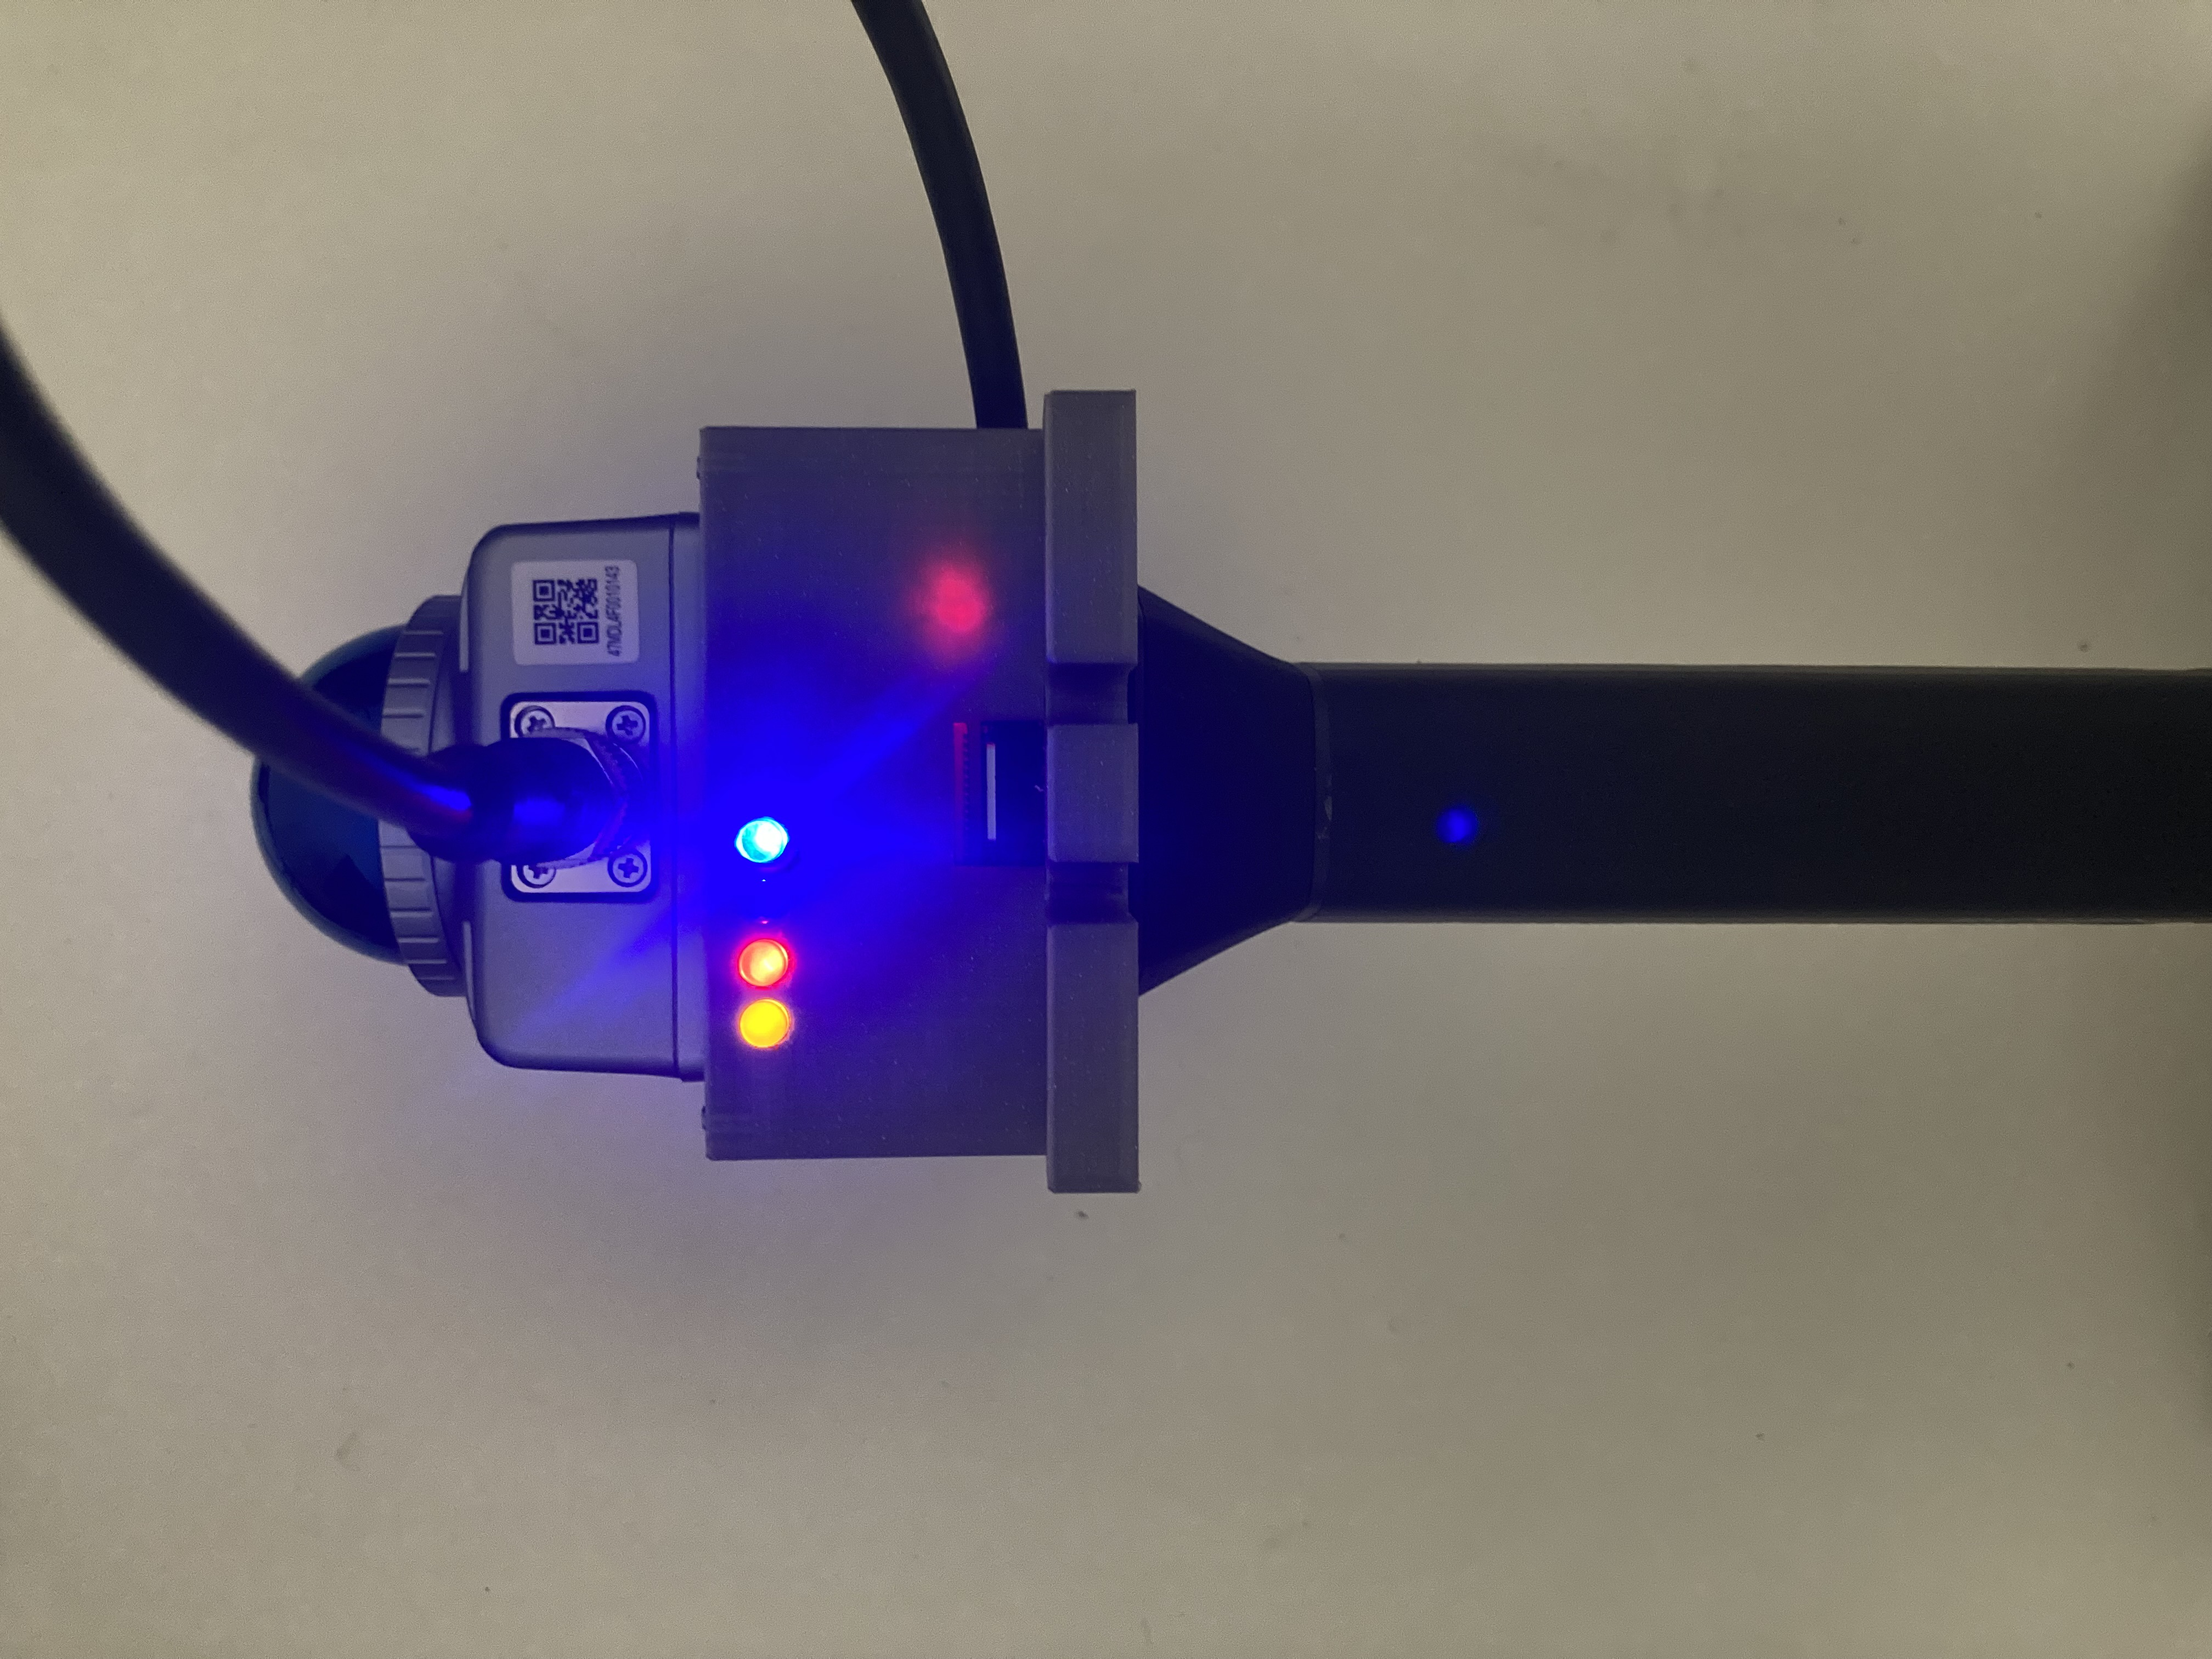
\includegraphics[width=\textwidth, angle = -90]{IMG_9499.jpg}
		\caption{MANDEYE DEV is showing by yellow and red light that it copies data from local memory to USB stick.}
		\label{fig:m42}
	\end{subfigure}
	\caption{MANDEYE DEV during stop/scan scanning.}
	\label{fig:mandeye_hardware4}
\end{figure}

\pagebreak
\section{Turn off device}
 After being finished using MANDEYE DEV make sure that no process is active (only blue light is on - figure \ref{fig:m22}). To turn the device off, press shortly RONIN grip button and then press longer RONIN grip button. All green lights on RONIN grip and blue light on MANDEYE main unit should turn off.
 \begin{figure}[H]
 	\centering
 	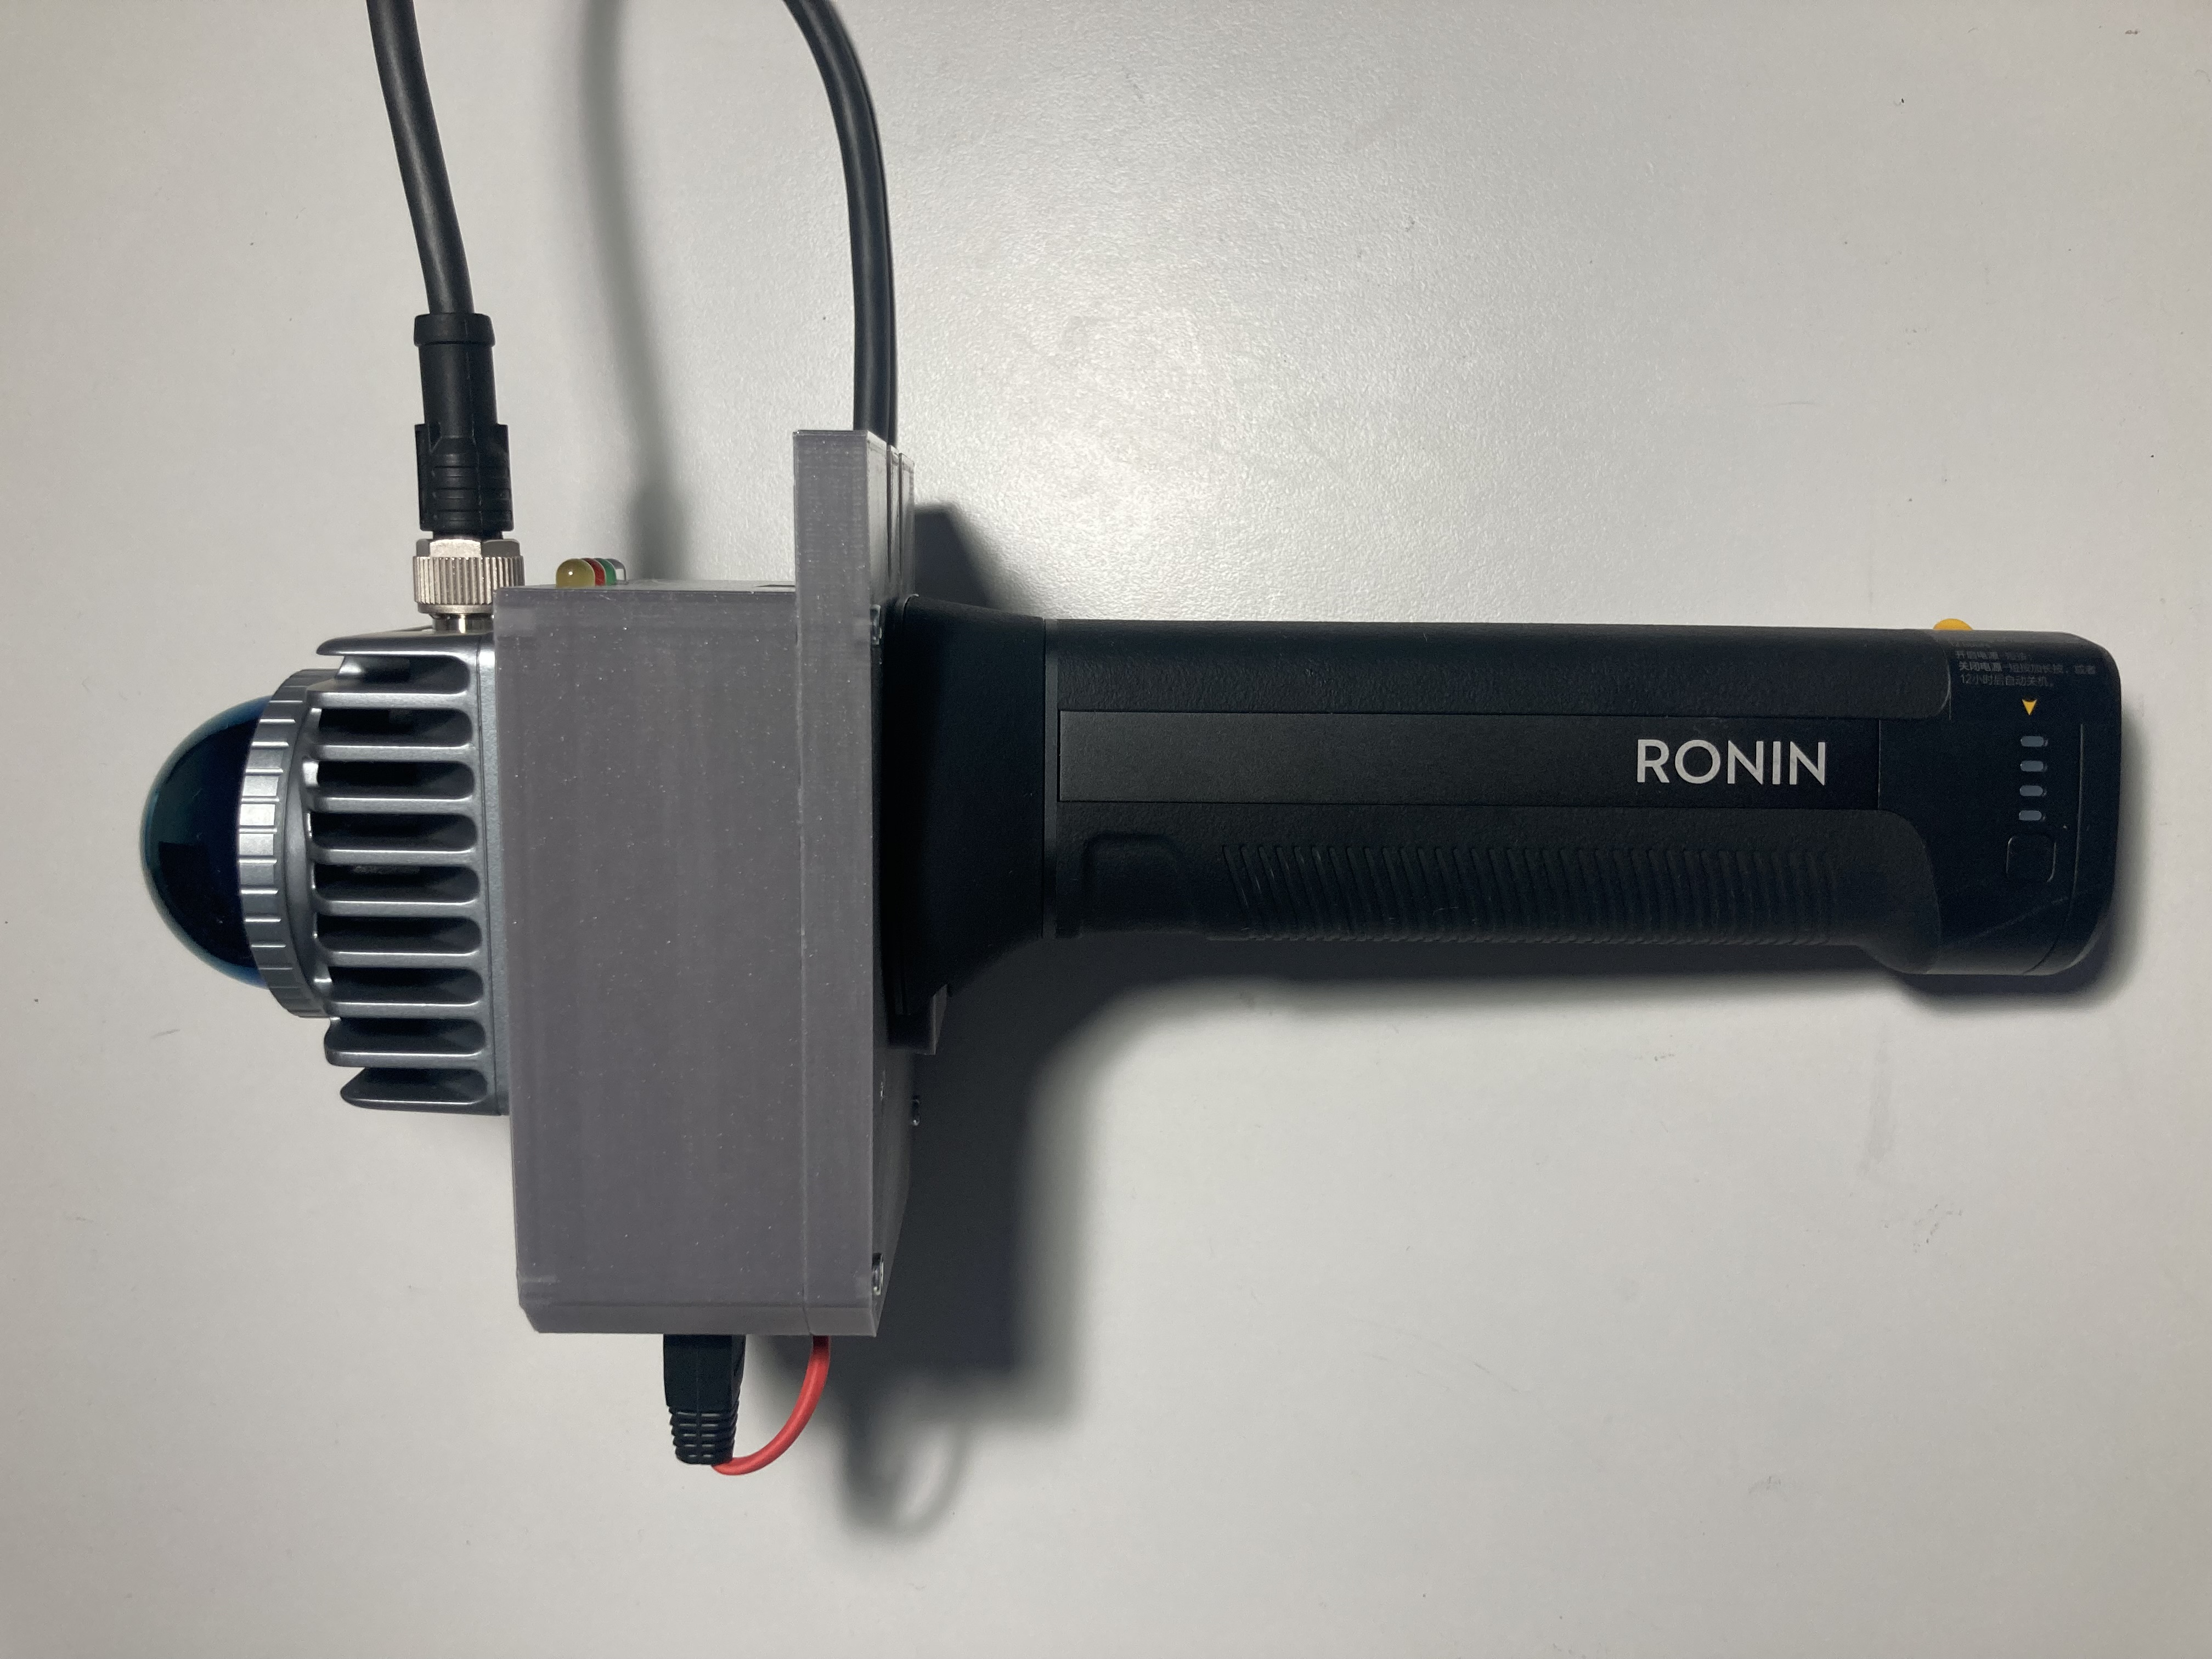
\includegraphics[width=\textwidth, angle = -90]{IMG_9483.jpg}
 	\caption{MANDEYE completely turned off. All RONIN lights are off.}
 	\label{fig:mandeye_hardware5}
 \end{figure}

\pagebreak
\section{Error indicators}
\label{section:errors}
MANDEYE DEV is capable of indicating two errors:
\begin{itemize}
	\item 1: "No USB drive", red light is blinking (figure \ref{fig:m61}),
	\item 2: "No communication with LiDAR", yellow and green lights are blinking (figure \ref{fig:m62}).
\end{itemize}

\begin{figure}[H]
	\centering
	\begin{subfigure}[b]{0.45\textwidth}
		\centering
		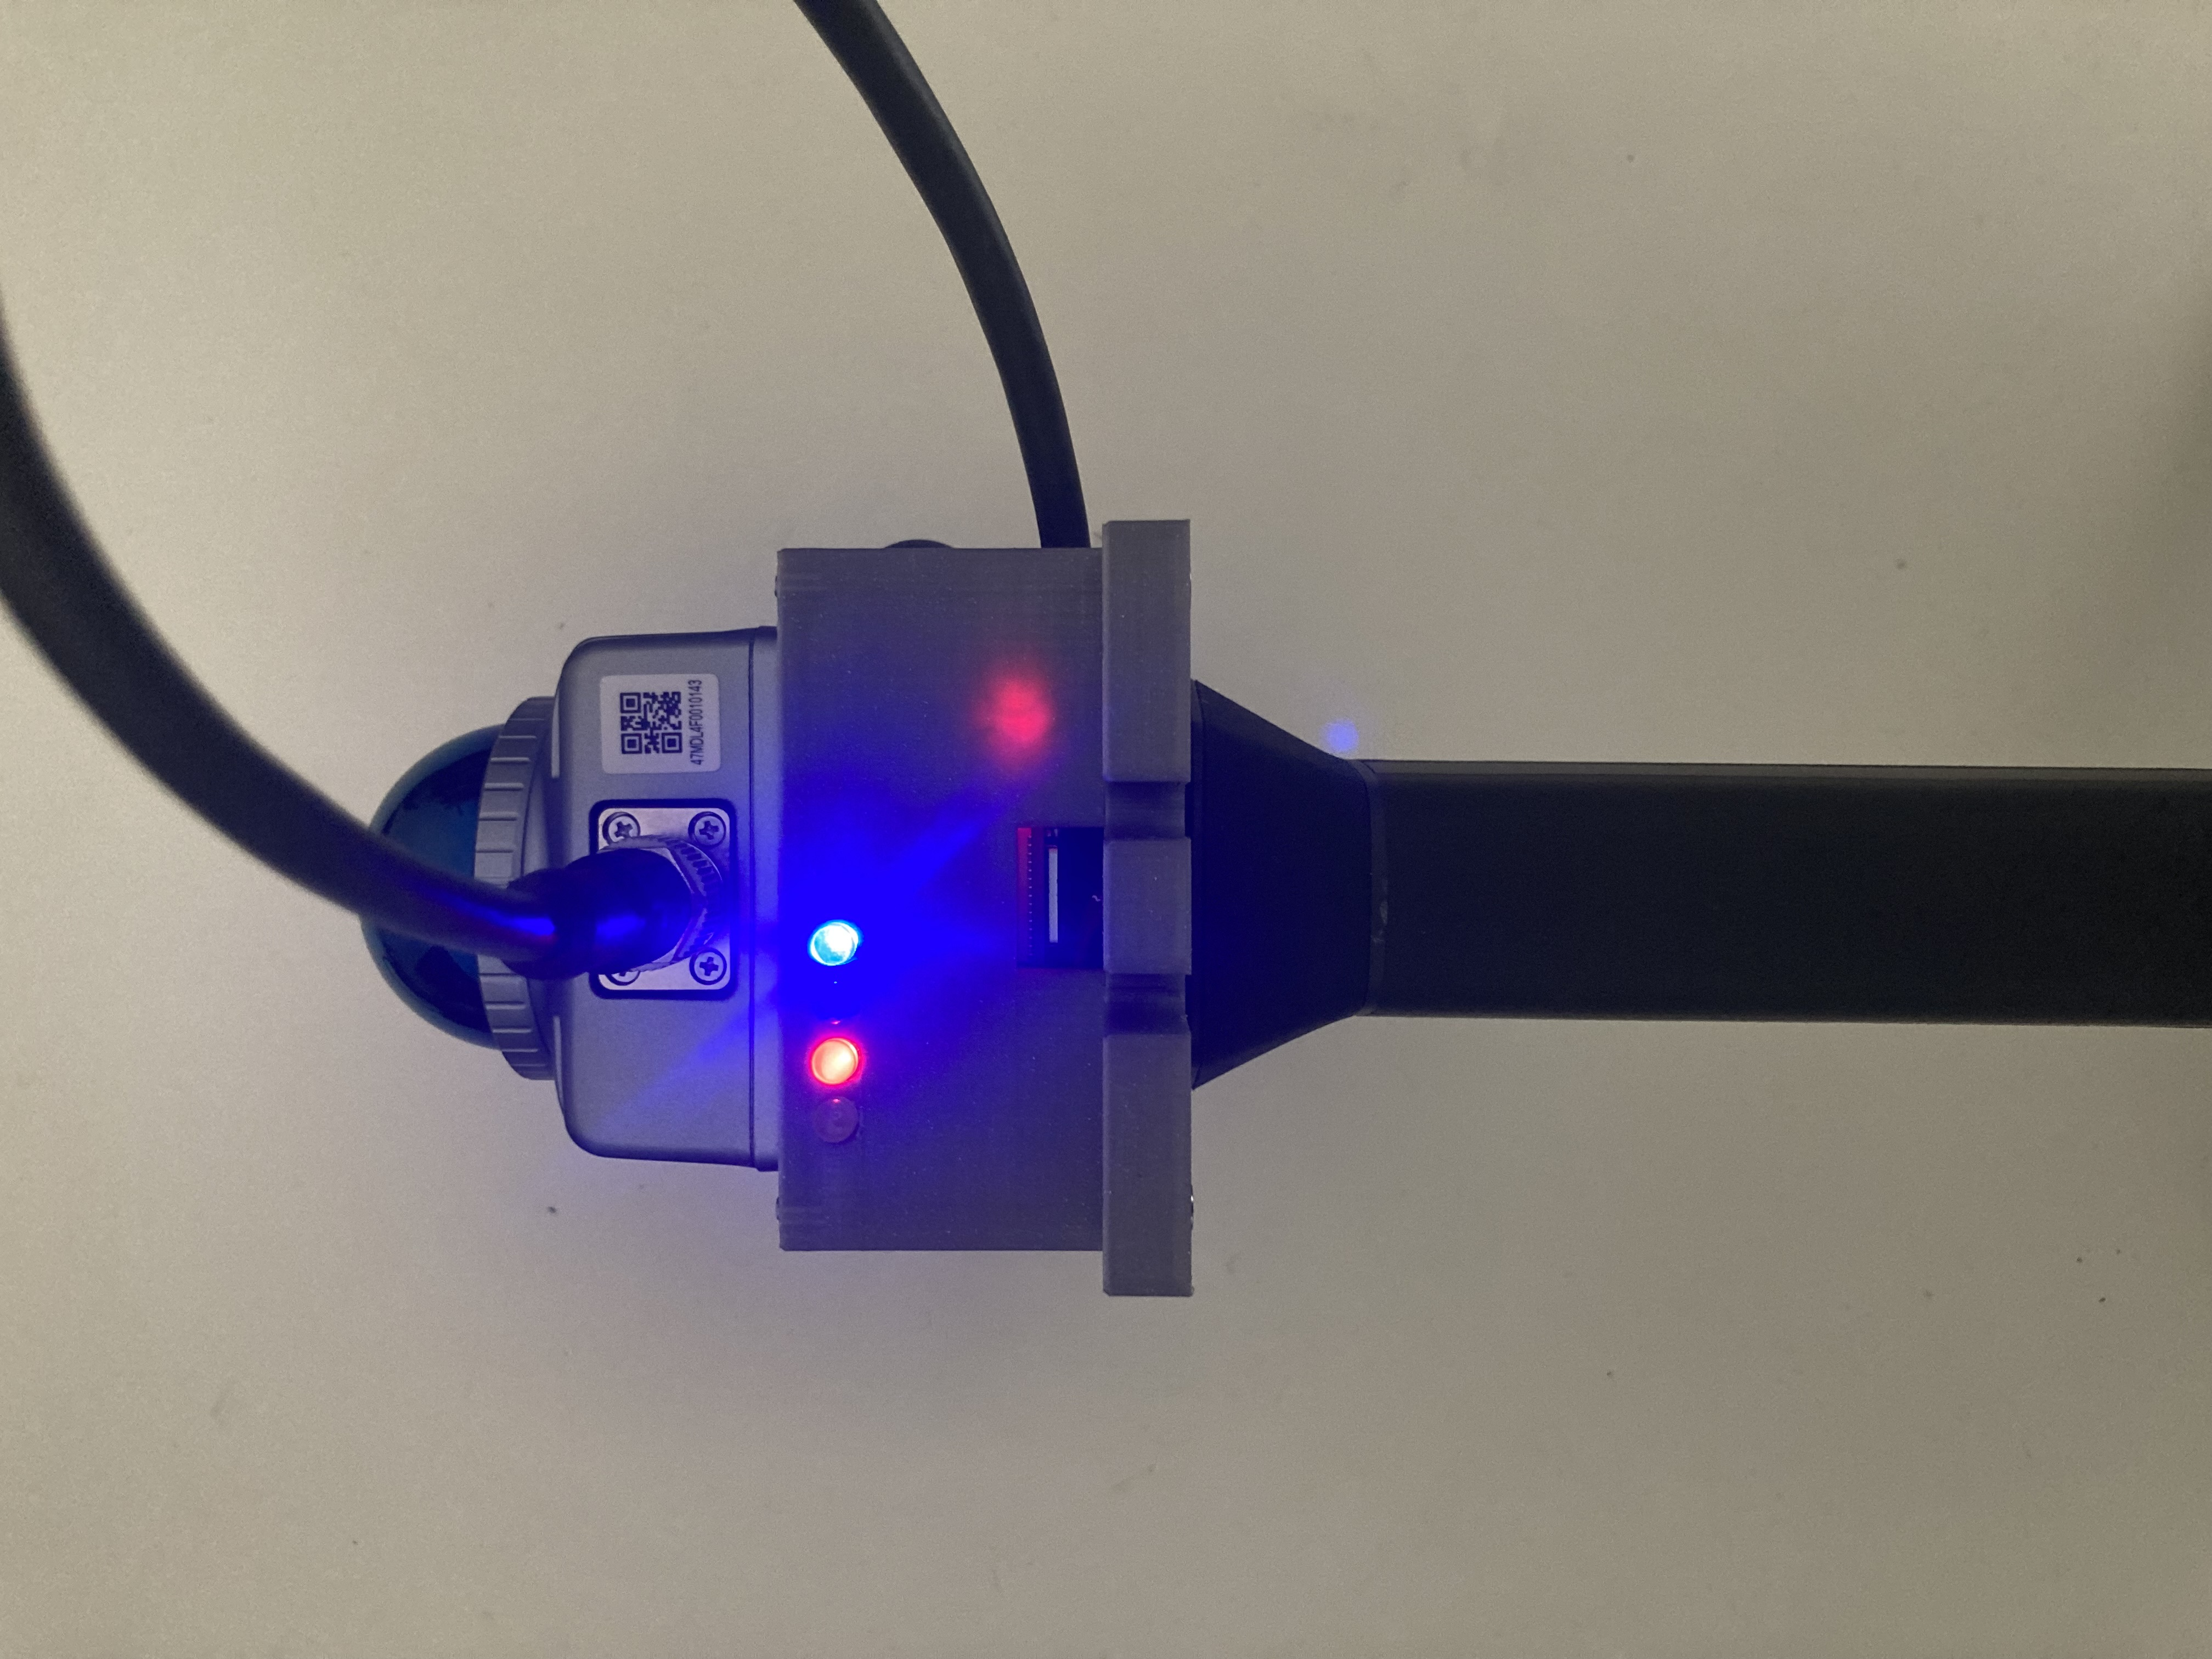
\includegraphics[width=\textwidth, angle = -90]{IMG_95011.jpg}
		\caption{MANDEYE DEV "no USB drive" error - blinking red light.}
		\label{fig:m61}
	\end{subfigure}
	\hfill
	\begin{subfigure}[b]{0.45\textwidth}
		\centering
		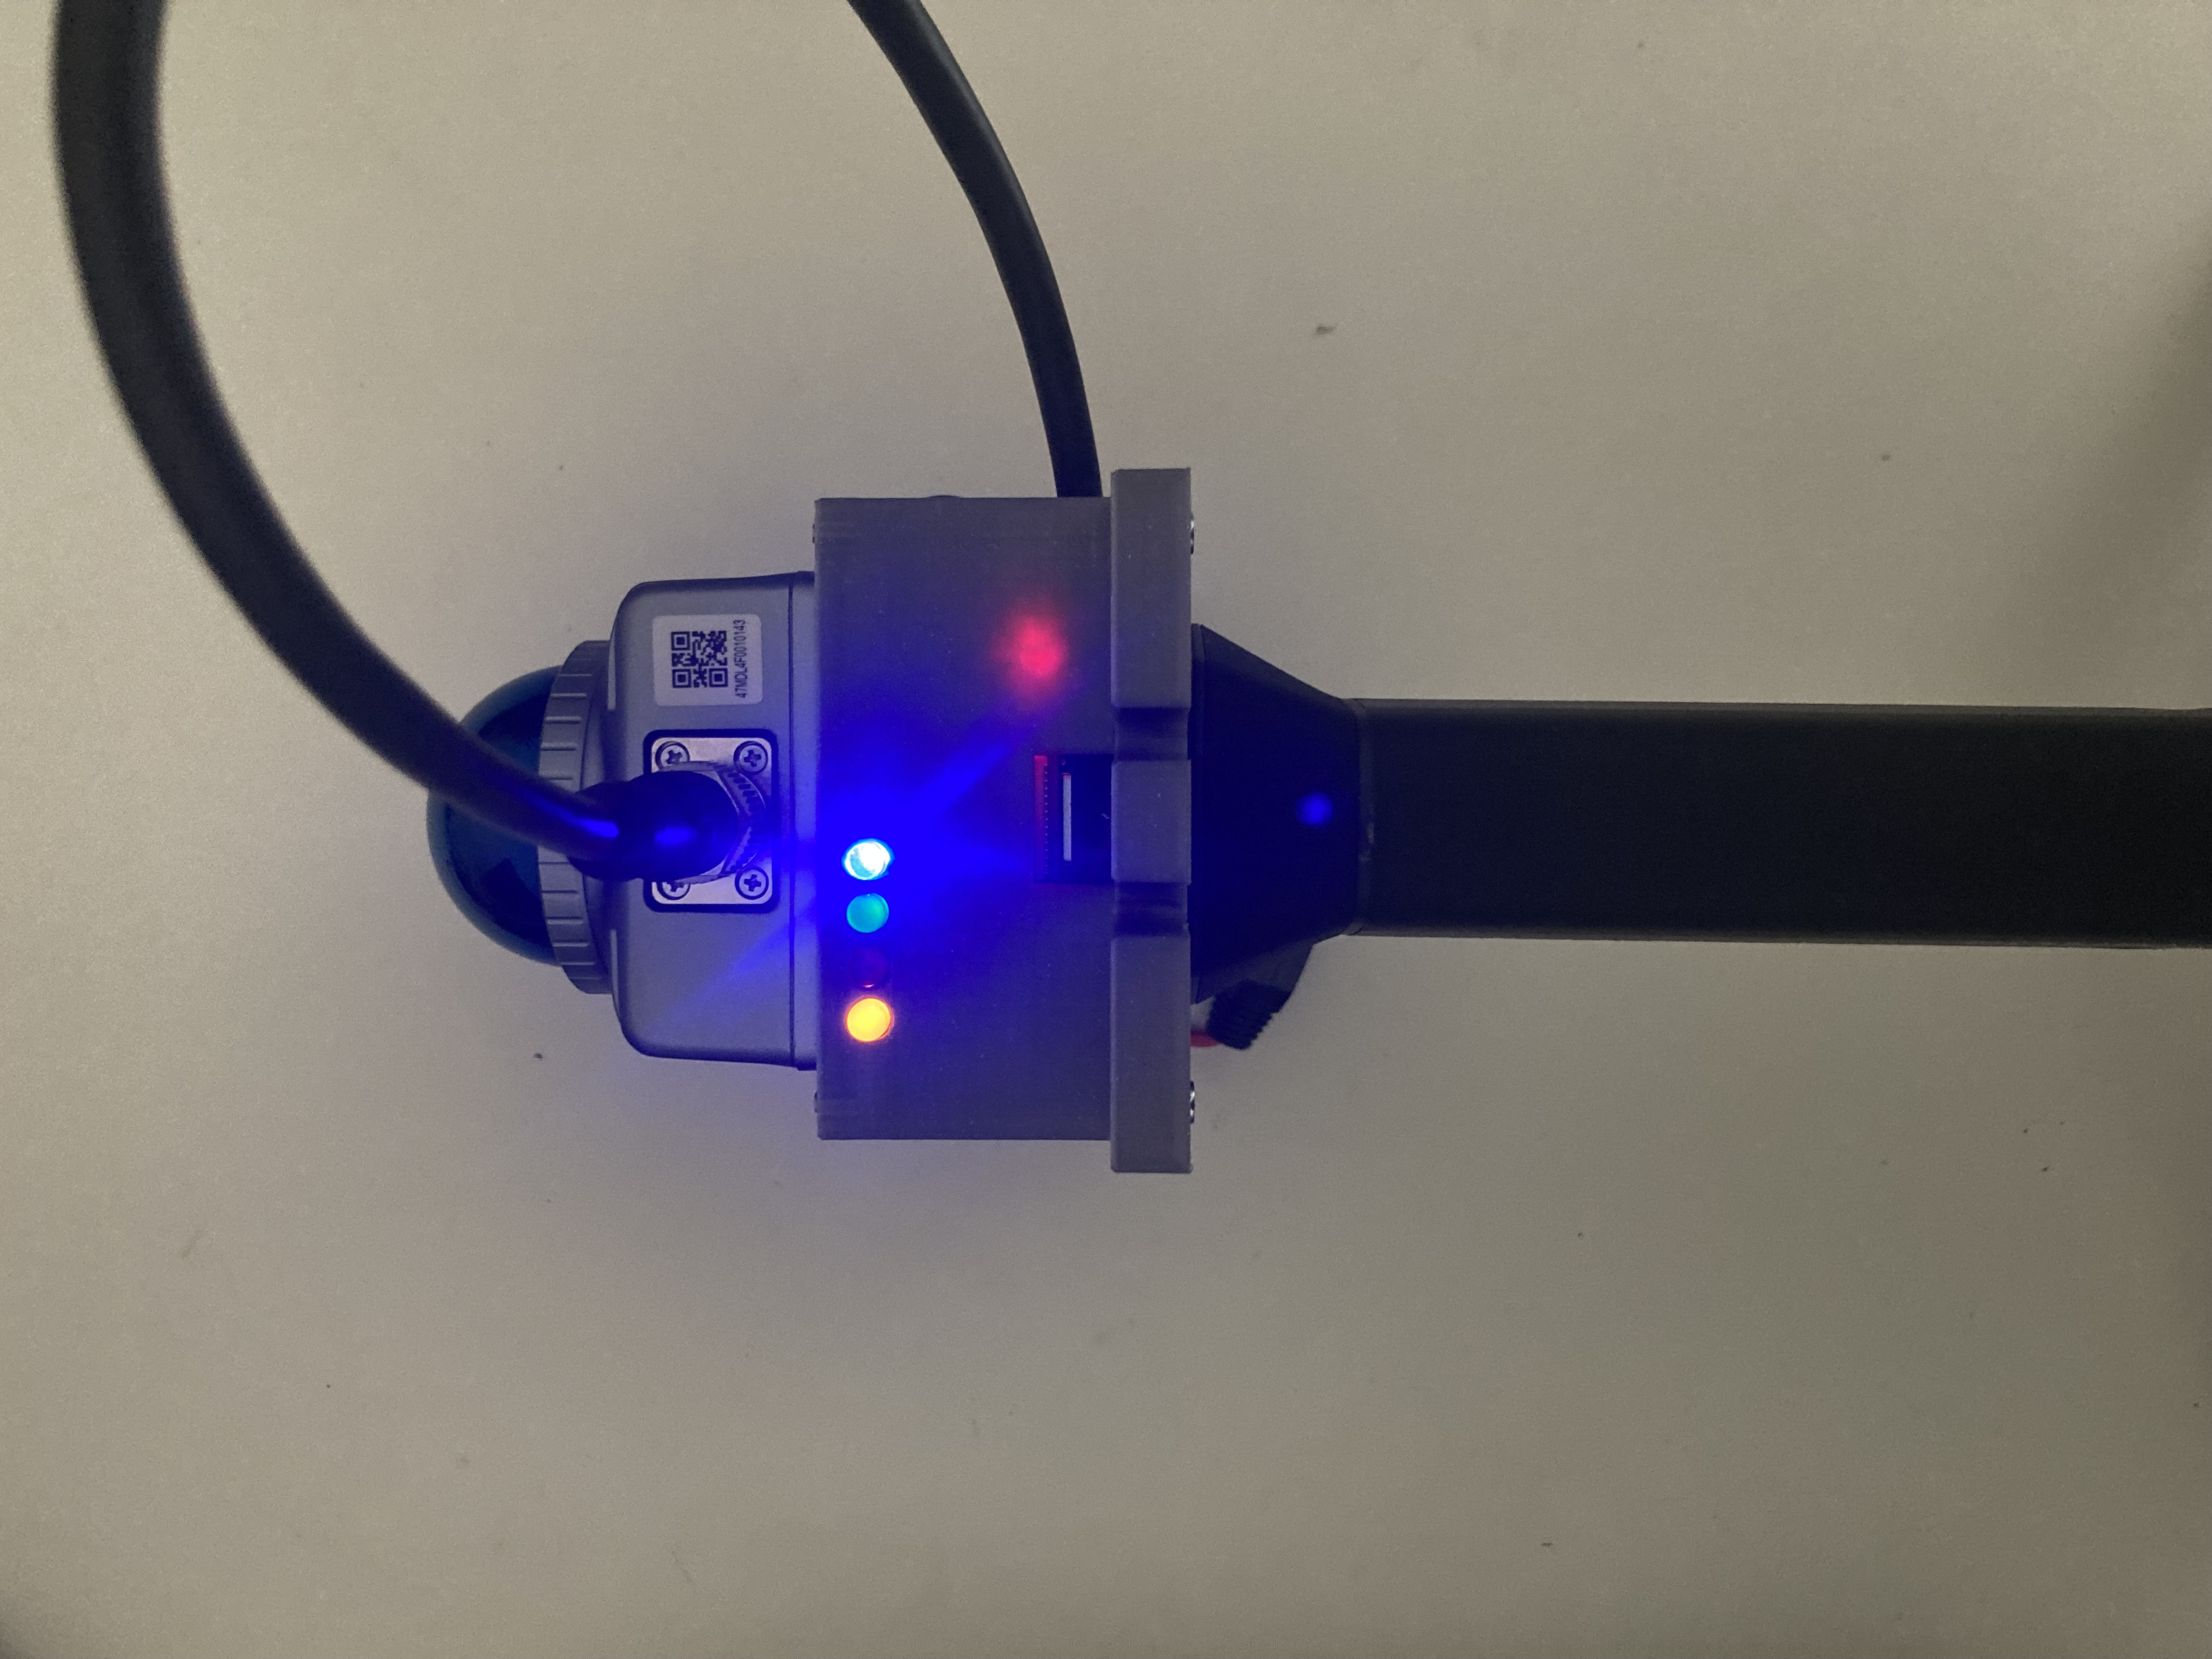
\includegraphics[width=\textwidth, angle = -90]{IMG_95021.jpg}
		\caption{MANDEYE DEV "no communication with LiDAR" error - blinking yellow and green lights.}
		\label{fig:m62}
	\end{subfigure}
	\caption{MANDEYE DEV error indicators.}
	\label{fig:mandeye_harware6}
\end{figure}
	
\section{Data structure on USB drive}
MANDEYE DEV starts with empty USB drive that has to be formatted as FAT, otherwise error "No USB drive" can appear.
Once MANDEYE DEV will be turned on it will create following data on USB drive:
\begin{itemize}
	\item $continousScanning\_0000$ (this is folder for continuous scanning data)
	\item $stopScans\_0000$ (this is folder for stop scan scanning data)
	\item $mandala\_manifest.txt$ (this is MANDEYE DEV internal file)
	\item version.txt (this file contains firmware version, so please check the title of this documentation if it is the same as on USB drive).
\end{itemize}
The more you operate with MANDEYE DEV the more $continousScanning\_0000$, $stopScans\_0000$ will appear. New folders are creating for each turn on of the MANDEYE DEV, so sometimes they can be empty.
Once you approach full USB drive, please remove all files from it.